\documentclass[11pt,twoside]{article}

% Text
\usepackage[utf8]{inputenc}

% Graphics
\usepackage{graphicx}
\usepackage{graphics}
\usepackage[dvipsnames, table]{xcolor}
\usepackage{tikz}
\usepackage{microtype}
\usepackage{setspace}
\usepackage{color, colortbl}

% Colors
\definecolor{Gray1}{gray}{0.9}
\definecolor{Gray2}{gray}{0.95}

% Geometry
\usepackage{geometry}
 \geometry{
 a4paper,
 left=25mm,
 right=25mm,
 top=30mm,
 bottom=25mm,
 heightrounded,
 headsep=7mm}

% URL
\usepackage{hyperref}

% Tables
\usepackage{tabu}
\usepackage{tabularx}
\usepackage{ltablex}
\usepackage{longtable}
\usepackage{float}
\usepackage{makecell}
\usepackage{array}

\begin{document}

\begin{center}
\thispagestyle{empty}

\includegraphics[scale=1.25]{Images/PolimiLogo}\\
\vspace{4cm}
\textbf{\Huge{Design Document}}\\
\vspace{1.5cm}
\textbf{\Large{Version 1.0}}\\
\bigskip \par
by \par
\large{Abdallah Alkhetiar}\\
\large{Daniel Bonardi}\\
\bigskip \bigskip
\large{\today}
\end{center}

\newpage

\setcounter{page}{1}
\begin{center}
\textbf{\Huge{Document details}}
\end{center}
\begin{table}[h!]
\begin{tabu} to \textwidth { |X[0.25,r,p] || X[0.75,l,p]| }
\hline

\textbf{Deliverable:} & DD \\
\hline
\textbf{Title:} & Design Document \\
\hline
\textbf{Authors:} & Abdallah Alkhetiar and Daniel Bonardi \\
\hline
\textbf{Version:} & 1.0 \\ 
\hline
\textbf{Date:} & \today \\
\hline
\textbf{Download page:} & \href{https://github.com/Zero3474/AlkhetiarBonardi.git}{\texttt{\color{blue}{github.com/Zero3474/AlkhetiarBonardi.git}}} \\
\hline
\textbf{Copyright:} & Copyright © 2025, Abdallah Alkhetiar and Daniel Bonardi \\
& – All rights reserved \\
\hline
\end{tabu}
\end{table}

\newpage

\tableofcontents

\newpage

\section{Introduction}
	\subsection{Purpose}
This design document outlines the architectural framework, user interface design, and other system components necessary to meet the functional and non-functional requirements described in the Requirement Analysis and Specification Document. \\
It also serves as a foundation for developers, testers, and stakeholders to understand the system's structure and ensures that the final implementation adheres to the defined goals. \\
The main purpose of the S\&C platform is to grant efficient and effective matchmaking between university students seeking experience through internships and companies offering them. The design aims to ensure:
\begin{itemize}
\item \textbf{Precision in matching}: The system adopts a sophisticated recommendation system to notify students about suitable internships, based on criteria such as skills and experiences.
\item \textbf{Smooth user experience}: The system shall grant its users the best experience by smoothly managing all internship-related workflows, including searching, application, selection, feedback collection, and monitoring of ongoing internships.
\item \textbf{Scalability}: The system's design shall accommodate future adjustments, such as advanced data analytics, integration with external tools, or even an expanded scope.
\end{itemize}

	\subsection{Scope}
\textbf{Students\&Companies} (S\&C) is an internship platform designed to connect students with companies based on skills, experiences, and interests. \\
The platform offers two main ways to establish connections:
\begin{itemize}
\item \textbf{Recommendation system}
\item \textbf{Proactive searching}
\end{itemize}
S\&C also supports the selection process  and gathers feedback on recommendations and provides spaces for users to address issues, share updates, and track internship progress.
More details can be found in the RASD document.
	\subsection{Definitions, acronyms, abbreviations}
DDoS: Distributed denial of service, an attack that floods a server with internet traffic.

	\subsection{Revision history}
Version 1.0 - WIP

	\subsection{Reference documents}
TBD

	\subsection{Document structure}
\textbf{Section 1: Introduction} \\
This section is presented with a brief overview of this document's content including the description of the purpose, the scope, and all the definitions, acronyms and abbreviations used.
\vspace{1\baselineskip} \\
\textbf{Section 2: Architectural design} \\
This section is presented with a detailed description of the architectural choices for the system, including a high-level description of the system and its components. In addition it is presented a detailed description of the deployment view and the main runtime views of the system.
\vspace{1\baselineskip} \\
\textbf{Section 3: User interface design} \\
This section is presented with a series of prototypes for the most important pages of the software to help graphic designers. Each image is accurately described to avoid any misunderstanding on the pages' available functionalities.
\vspace{1\baselineskip} \\
\textbf{Section 4: Requirements traceability} \\
This section is highly dependent on the RASD, as it provides a complete mapping of both functional and non-functional requirements described in that document, with the modules introduced and described in this document.
\vspace{1\baselineskip} \\
\textbf{Section 5: Implementation, integration and test plan} \\
The last section describes the procedures followed for implementing, integrating and testing the components of the platform.

\newpage

\section{Architectural design}
	\subsection{Overview}	
The S\&C design is based on two architectural choices:
\begin{itemize}
\item A 3 tier architecture
\item A thin-client model
\end{itemize}
First of all the 3 tier architecture is built using 3 layers:
\begin{itemize}
\item \textbf{Presentation layer}: This layer is in charge of providing all the user interfaces for users to interact with the system.
\item \textbf{Application layer}: This layer implements the core of the business logic and processes all the requests sent from the presentation layer.
\item \textbf{Data layer}: This layer is responsible of managing all the data storage.
\end{itemize}
The choice of the 3 tier architecture what made to grant these key concepts:
\begin{itemize}
\item \textbf{Modularity}: Components are designed address a specific function required by the system, also making it easier to perform maintenance.
\item \textbf{Scalability}: Since each module function independently from the others, adding or removing feature should be easier.
\item \textbf{Security}: By implementing a secure communication protocol, users should not be worried about their sensitive data being stolen.
\end{itemize}
The thin-client approach instead, ensures the smoothest experience for the users, by keeping the client-side of the application as lightweight as possible. With this approach the client shall focus solely on the rendering of the user interface and the management of basic interactions, the rest of the computation happens on the server-side.\\
To sum it up, in the client there is only the presentation layer, while the application and data layer are in the server.

	\subsection{Component view}
To make it easier to understand component view, we decided to divide it into 3 diagrams. The first represents a high-level view that distinguishes the client-side from the server-side components. The other 2 diagrams represent a more detailed version of the components presented in the server-side in the first diagram.

		\subsubsection{High level component view}
In the following diagram it is shown how the client-side interacts with the server side through the exposed interfaces.\\
We can clearly see the 2 sides:
\begin{itemize}
\item \textbf{Client-side}: Since the in the client-side we only have the presentation layer, we can see that on the left of the diagram there are the Users, that can either be accessing the application through a web browser or a mobile device.
\item \textbf{Server-side}: On the server-side instead, we have both the application and data layer so we have the most important subsystems of the entire application:
	\begin{itemize}
	\item \textit{Internship management}: Which is the actual biggest component which manages all the actions that involve internships.
	\item \textit{Account management}: Which simply manages all the interactions that require some data regarding a user.
	\end{itemize}
\end{itemize}

\begin{figure}[H]
\centering
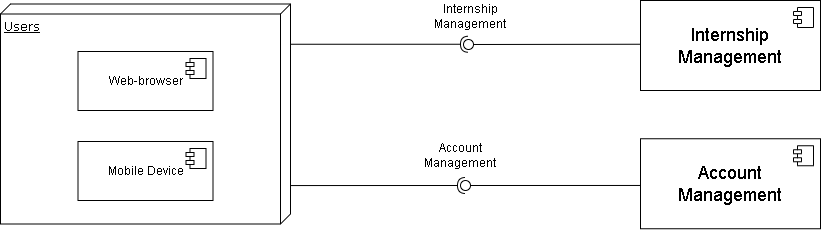
\includegraphics[width=0.9\textwidth]{Images/Component}
\caption{High level component view}\label{Component}
\end{figure}
\vspace{\baselineskip}

		\subsubsection{Internship management diagram}
The following diagram shows how the subsystem Internship Management is composed and how its modules communicate with external ones. This subsystem contains 6 modules:	
\begin{itemize}
\item \textbf{Proactive search}: Allows student to search for specific internship.
\item \textbf{Internship archival}: Allows companies to archive an internship, and show it on their profile.
\item \textbf{Feedback}: Allows user to send a feedback.
\item \textbf{Internship creation}: Allows companies to create an internship, and for this reason it needs to interact with the "Recommendation system" component to notify the compatible students.
\item \textbf{Complaints}: Allows user to file a complaint, and it also needs to interact with the "Notification system" to notify the universities.
\item \textbf{Form management}: Manages all the stages of a form, from its creation to the correction, and for this reason it needs to interact with the "Ranking system" component.
\end{itemize}
At the same time all components, external or internal to the subsystem, must interact with the DBMS to access all the data required for the interaction.
\newpage

\begin{figure}[H]
\centering
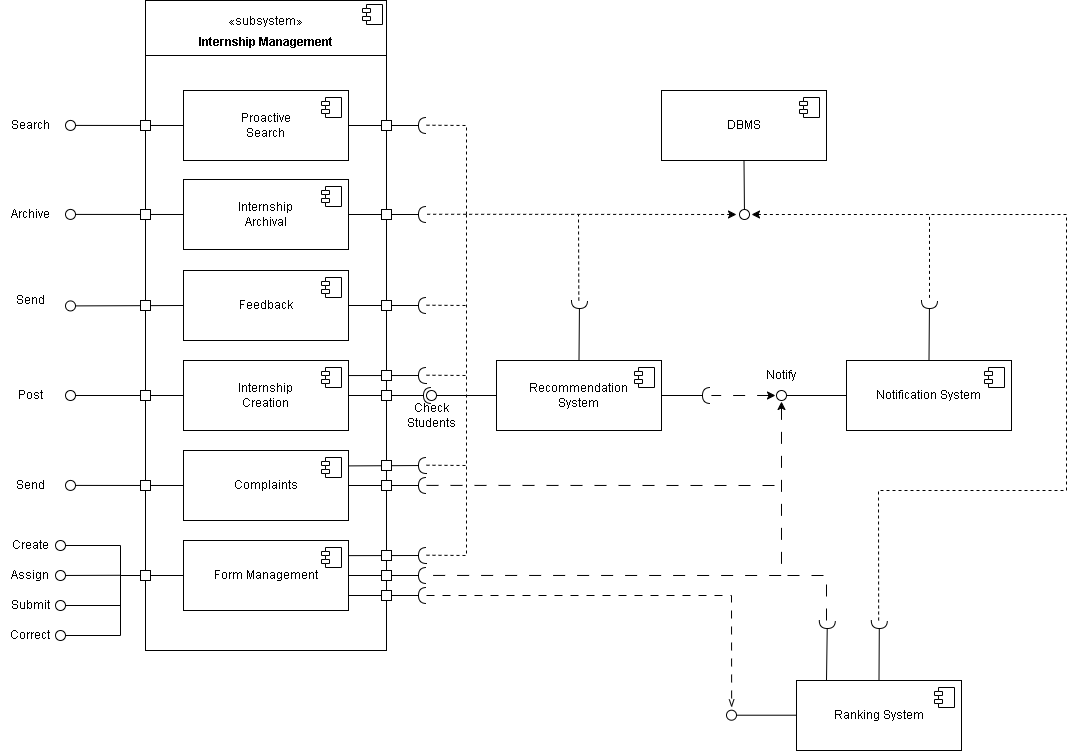
\includegraphics[width=0.95\textwidth]{Images/Component2}
\caption{Internship management diagram}\label{Component2}
\end{figure}
		
		\subsubsection{Account management diagram}
The following diagram shows how the subsystem Account Management is composed and how its modules communicate with external ones. This subsystem contains only 2 modules:
\begin{itemize}
\item \textbf{Student manager}: Allows student to sign up, login, add a CV and update their profile.
\item \textbf{Company manager}: Allows a company to sign up, login and update their profile.
\end{itemize}
In both cases the component need to access both the "Authentication" component to safely complete the login and sign up processes, and also the DBMS to manage all the required data.

\begin{figure}[H]
\centering
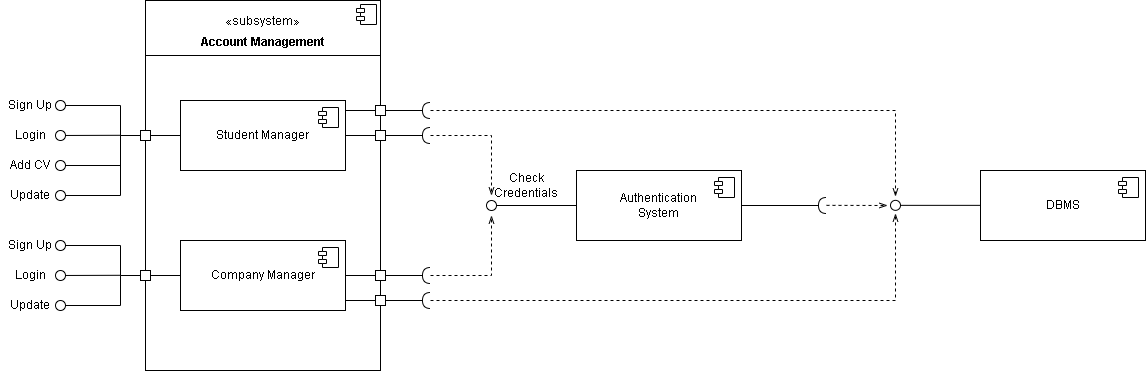
\includegraphics[width=0.95\textwidth]{Images/Component3}
\caption{Account management diagram}\label{Component3}
\end{figure}

\newpage

	\subsection{Deployment view}
\begin{figure}[H]
\centering
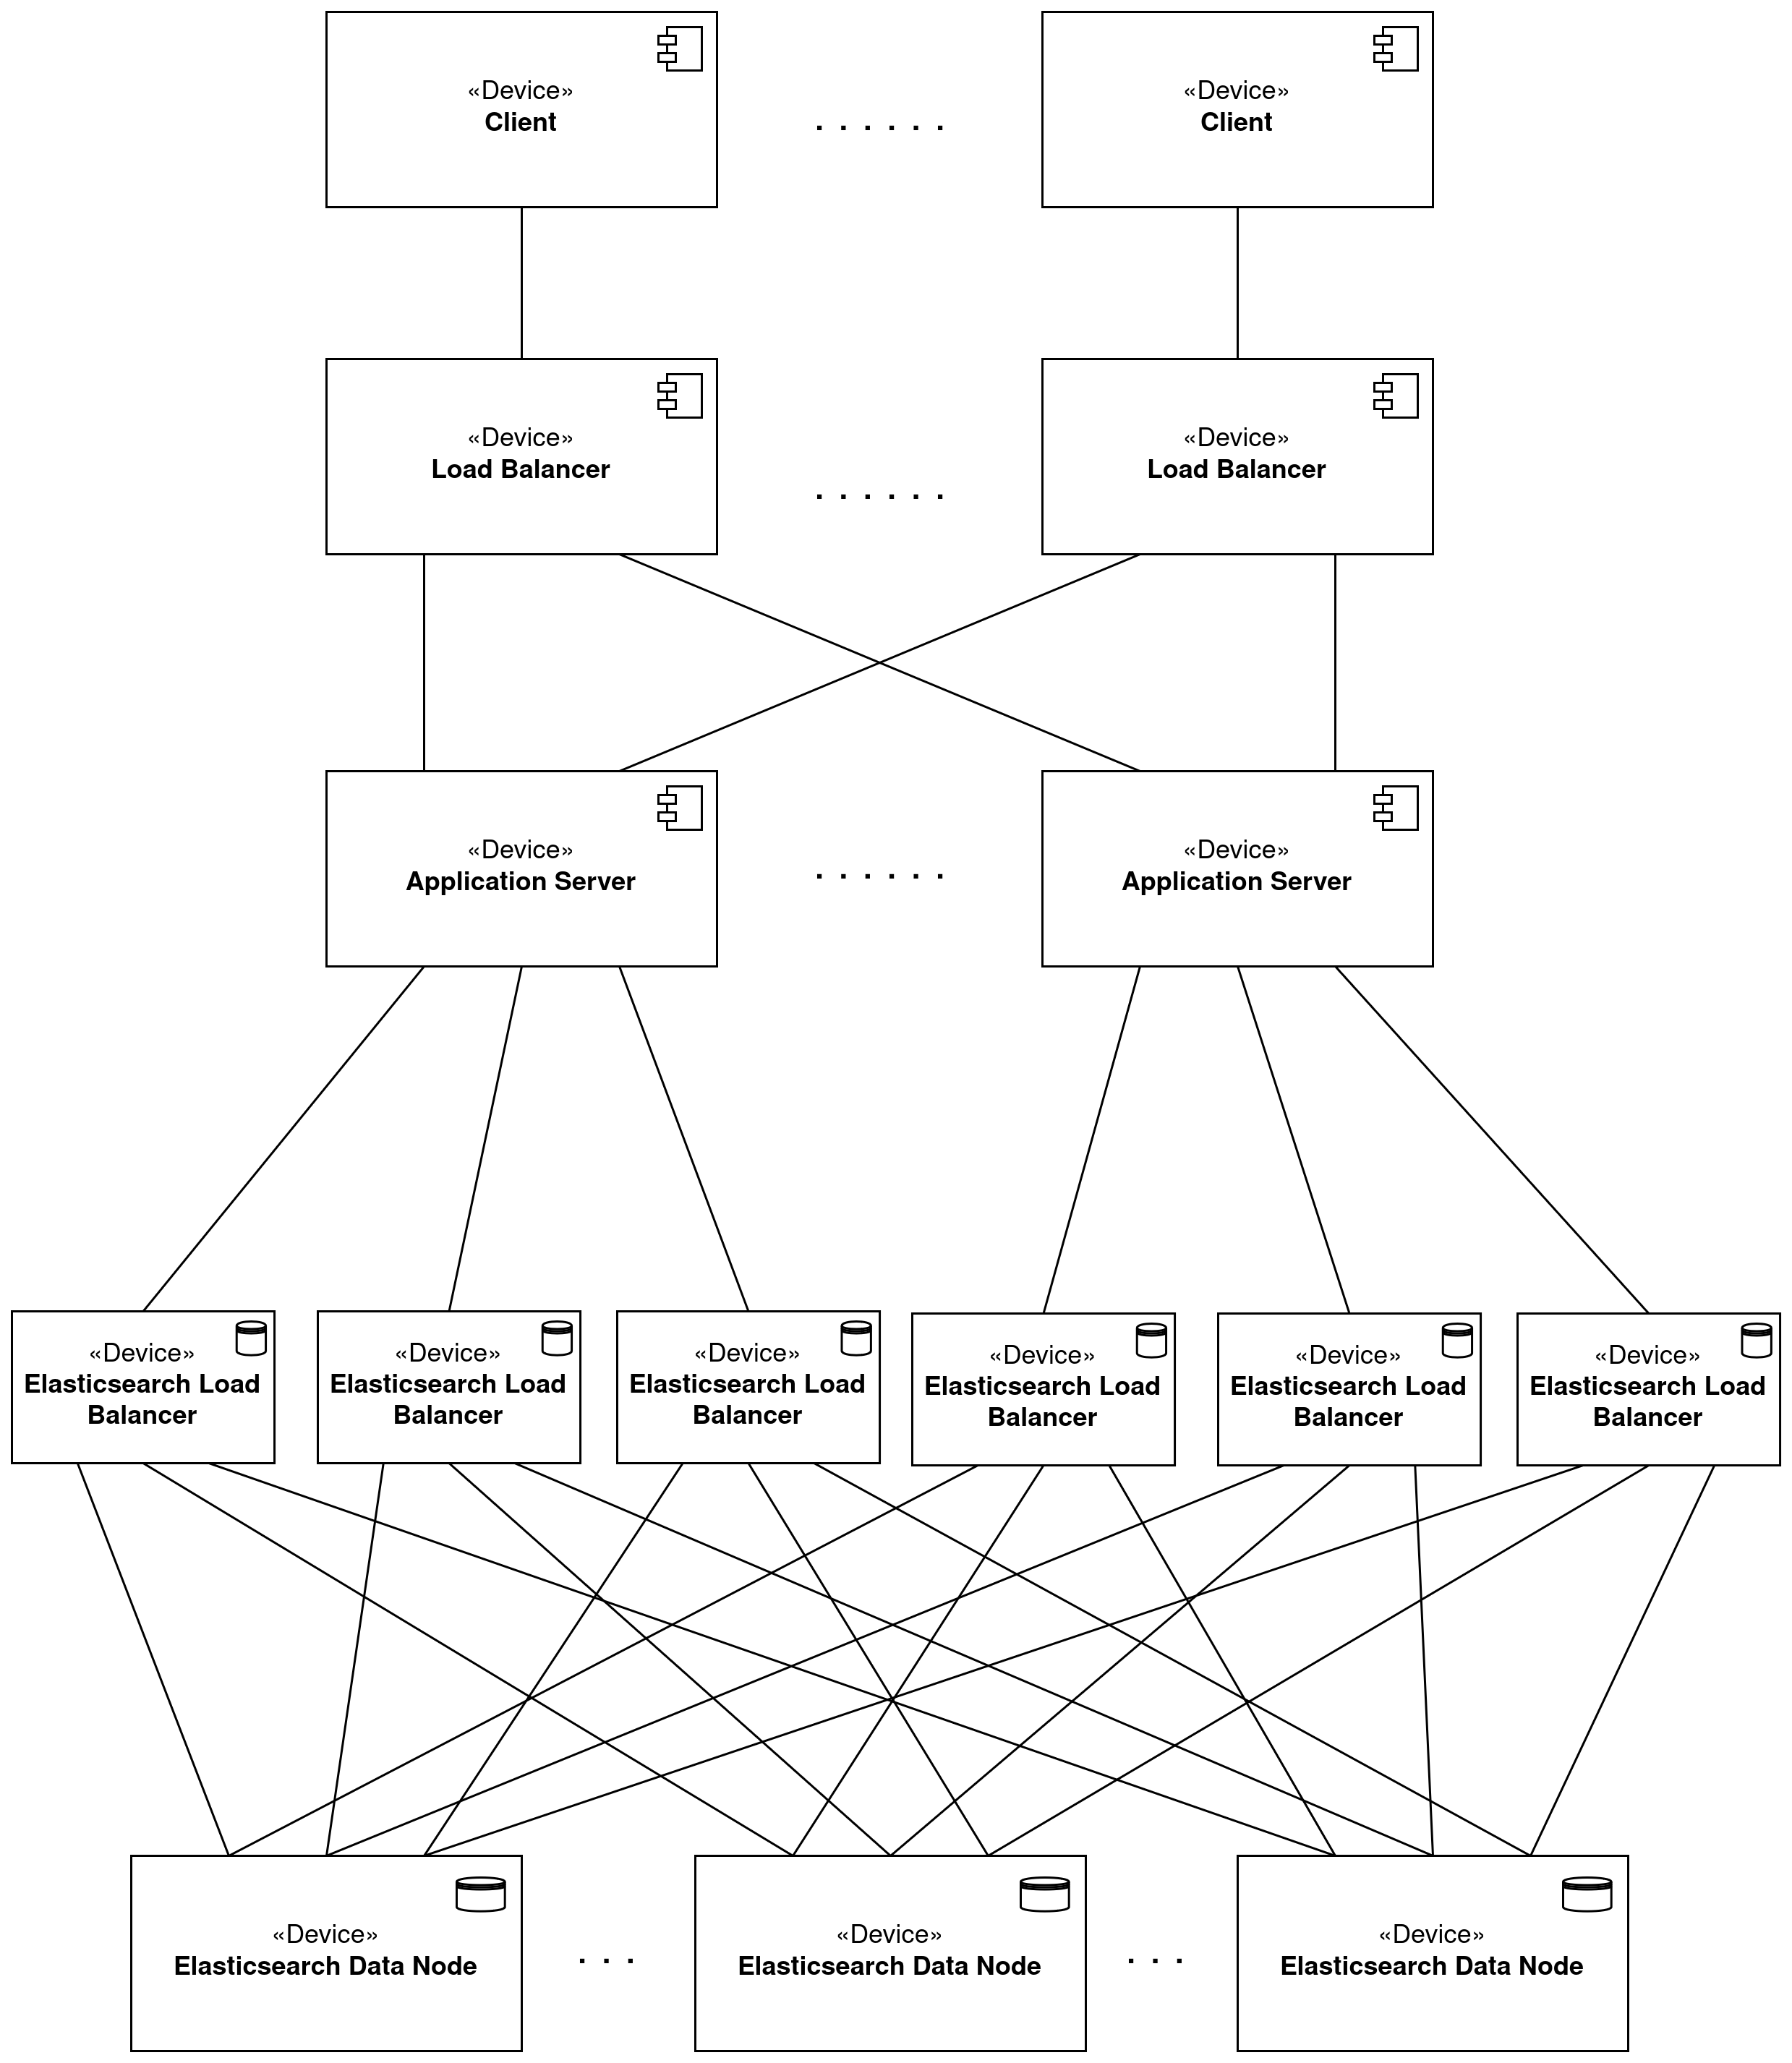
\includegraphics[width=0.95\textwidth]{Images/Deployment_view}
\caption{Deployment View Diagram}\label{Deployment_view}
\end{figure}

\newpage

The deployment view diagram provides a detailed view of the physical architecture of the system, describing how different elements interact with each other and where they are positioned. \\
Going with an Elasticsearch database will allow us to fully utilize the power of text search and reverse indexing to be able to provide really fast and accurate search results for the users. Since the system has the main function of acting as a recommender system, Elasticsearch seems like the best database technology to go with since it's quite suitable for the implementation of the AI recommender agent. \\
For what concerns scalability and availability, the inclusion of multiple load balancers and application server instances guarantees higher availability in case of device failures and thus avoiding single point of failures. This can also be seen with how the internal Elasticsearch load balancers and data nodes are replicated, three instances were chosen because that was the recommended nummber by the elasticsearch webpage for commercial databases, this replication not only is useful for higher avilability but even for better scalability thanks to the sharding approach that is implemented by default by the database technology. \\
A firewall shall also be implemented within the load balancers between the clients and the application servers, to provide protection against DDoS attacks and similar threats. \\
Now for a short describtion of how the system will work according to the diagram. Users will connect to a load balancer instance that will be chosen with respect to their geographical positions (to minimize latency), these load balancers will redirect user requests to the "best" application server instance according to a load balancing policy. After that, the server will send the request to the main elasticsearch load balancer which could change depending on the availability of the instances. And finally, the request will be completed by an appropriate data node that will handle the execution of the request and send back the result. \\
With this approach, no single point of failures exist and high availability and scalability are guaranteed, the only issues lie with the difficulty of implementing the load balancing policies of the external devices. \\

	\subsection{Runtime view}
With the following sequence diagrams, we are going to explain and represent all the interactions that happen between the components of the S\&C system. But since this representation is still a high-level description of interactions, the function names, parameters, results, errors, and other smaller details will be modified or added during the development phase.

		\subsubsection{Login}
In the login process, the user interacts with the \textit{Web Application} to login in his account. After adding the required information, the data is sent to the \textit{Account Manager} that checks if the credentials are correct through the \textit{Authentication System} that accesses the \textit{DBMS}. If the credentials are correct, the user is shown the home page, otherwise he is shown a message error and can try to login again.

\begin{figure}[H]
\centering
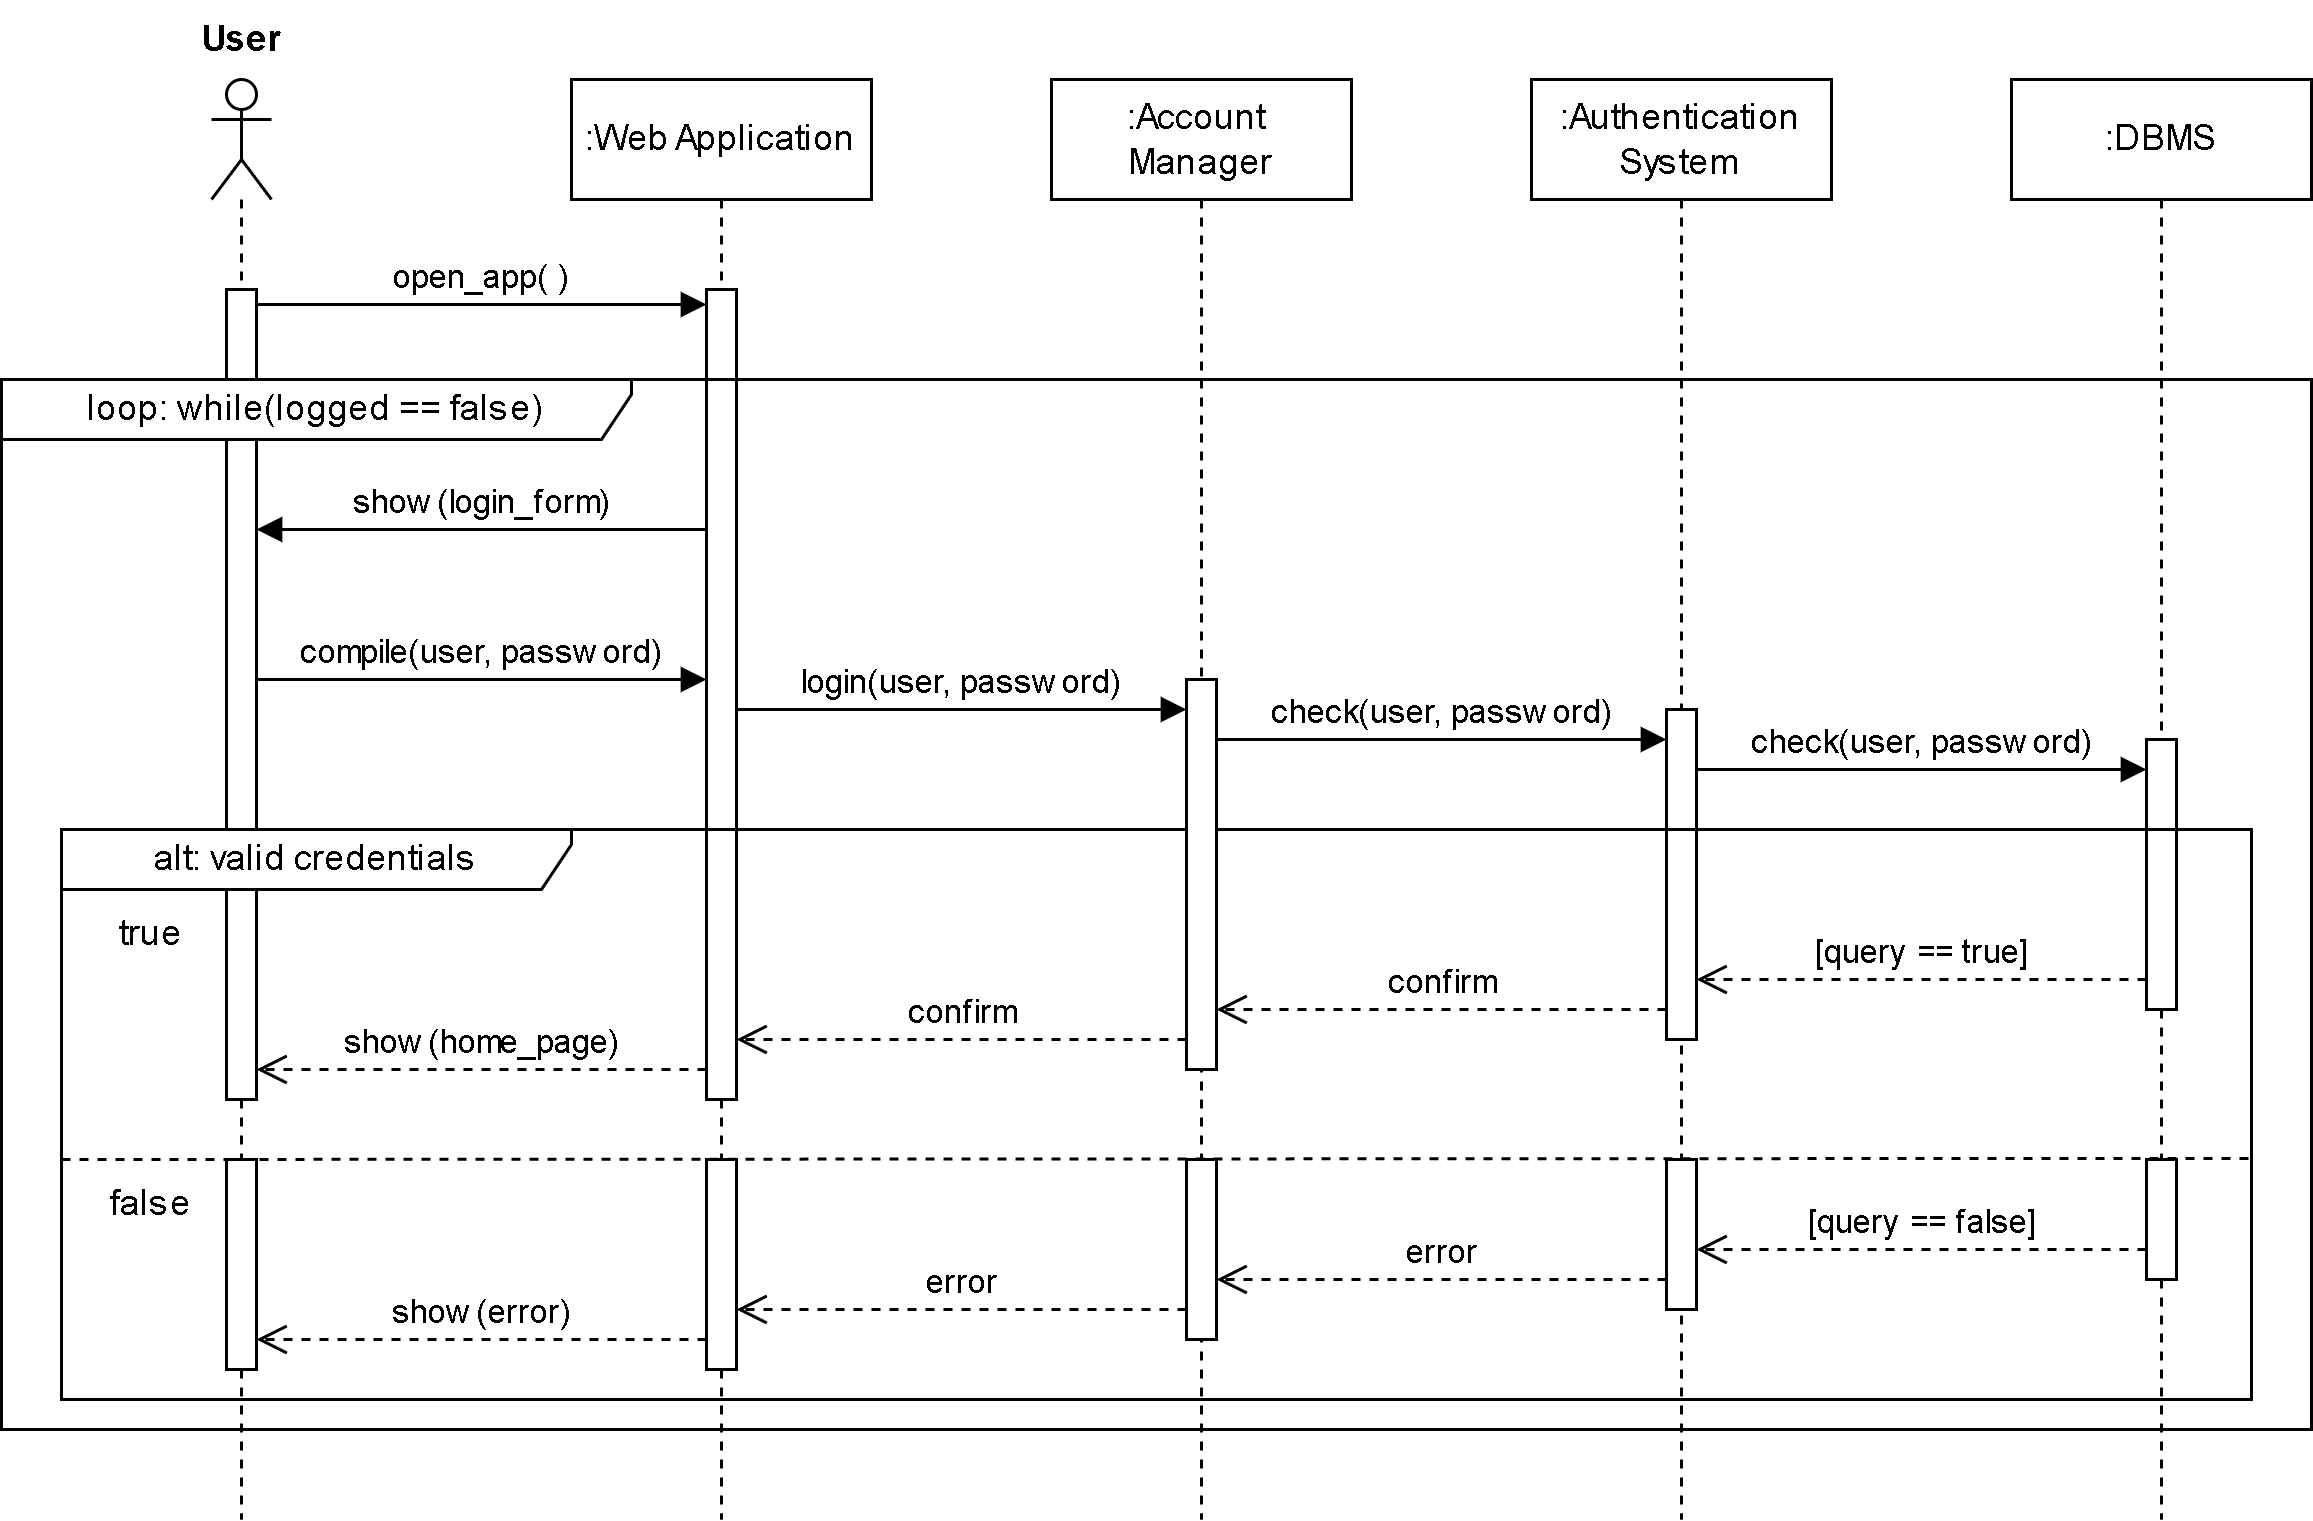
\includegraphics[width=0.95\textwidth]{Images/Seq1}
\caption{Login sequence diagram}\label{Seq1}
\end{figure}

\newpage

		\subsubsection{Sign up}
In the sign up process, the user interacts with the \textit{Web Application} to create a new account. When entering the application, the user is presented with the login page, so he needs to request for the sign up page. After adding the required information, the data is sent to the \textit{Account Manager} that checks if the credentials already exist in the data base. If the given information are correct, the user is shown the loin page, otherwise he is shown a message error and can try to create his account again.	
		
\begin{figure}[H]
\centering
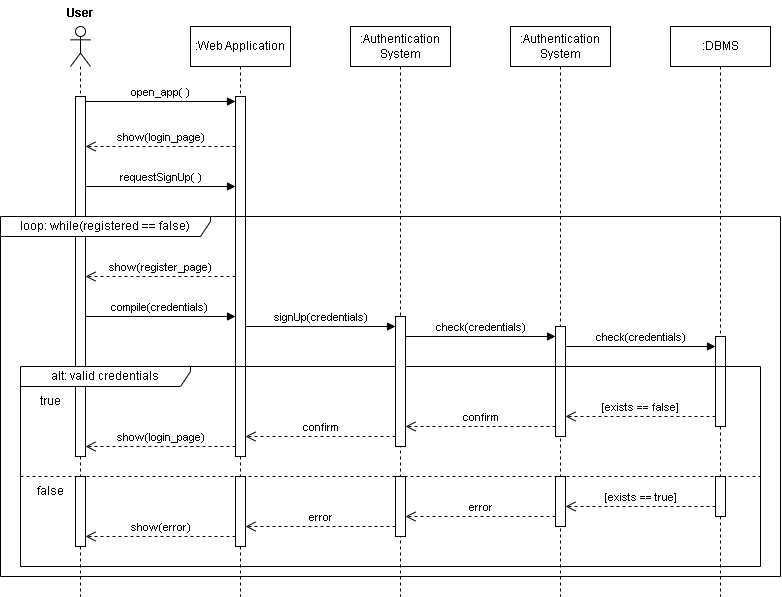
\includegraphics[width=0.95\textwidth]{Images/Seq2}
\caption{Sign up sequence diagram}\label{Seq2}
\end{figure}

\newpage

		\subsubsection{Internship creation}
In the internship creation process, a company interacts with the \textit{Web Application} to post about a new internship. When entering all the correct information, the \textit{Manage Internship} module interacts with the \textit{Recommendation System} to identify all the student that are deemed compatible with the internship. Once the system has gotten the list, all the specified students are notified through the \textit{Notification System}.

\begin{figure}[H]
\centering
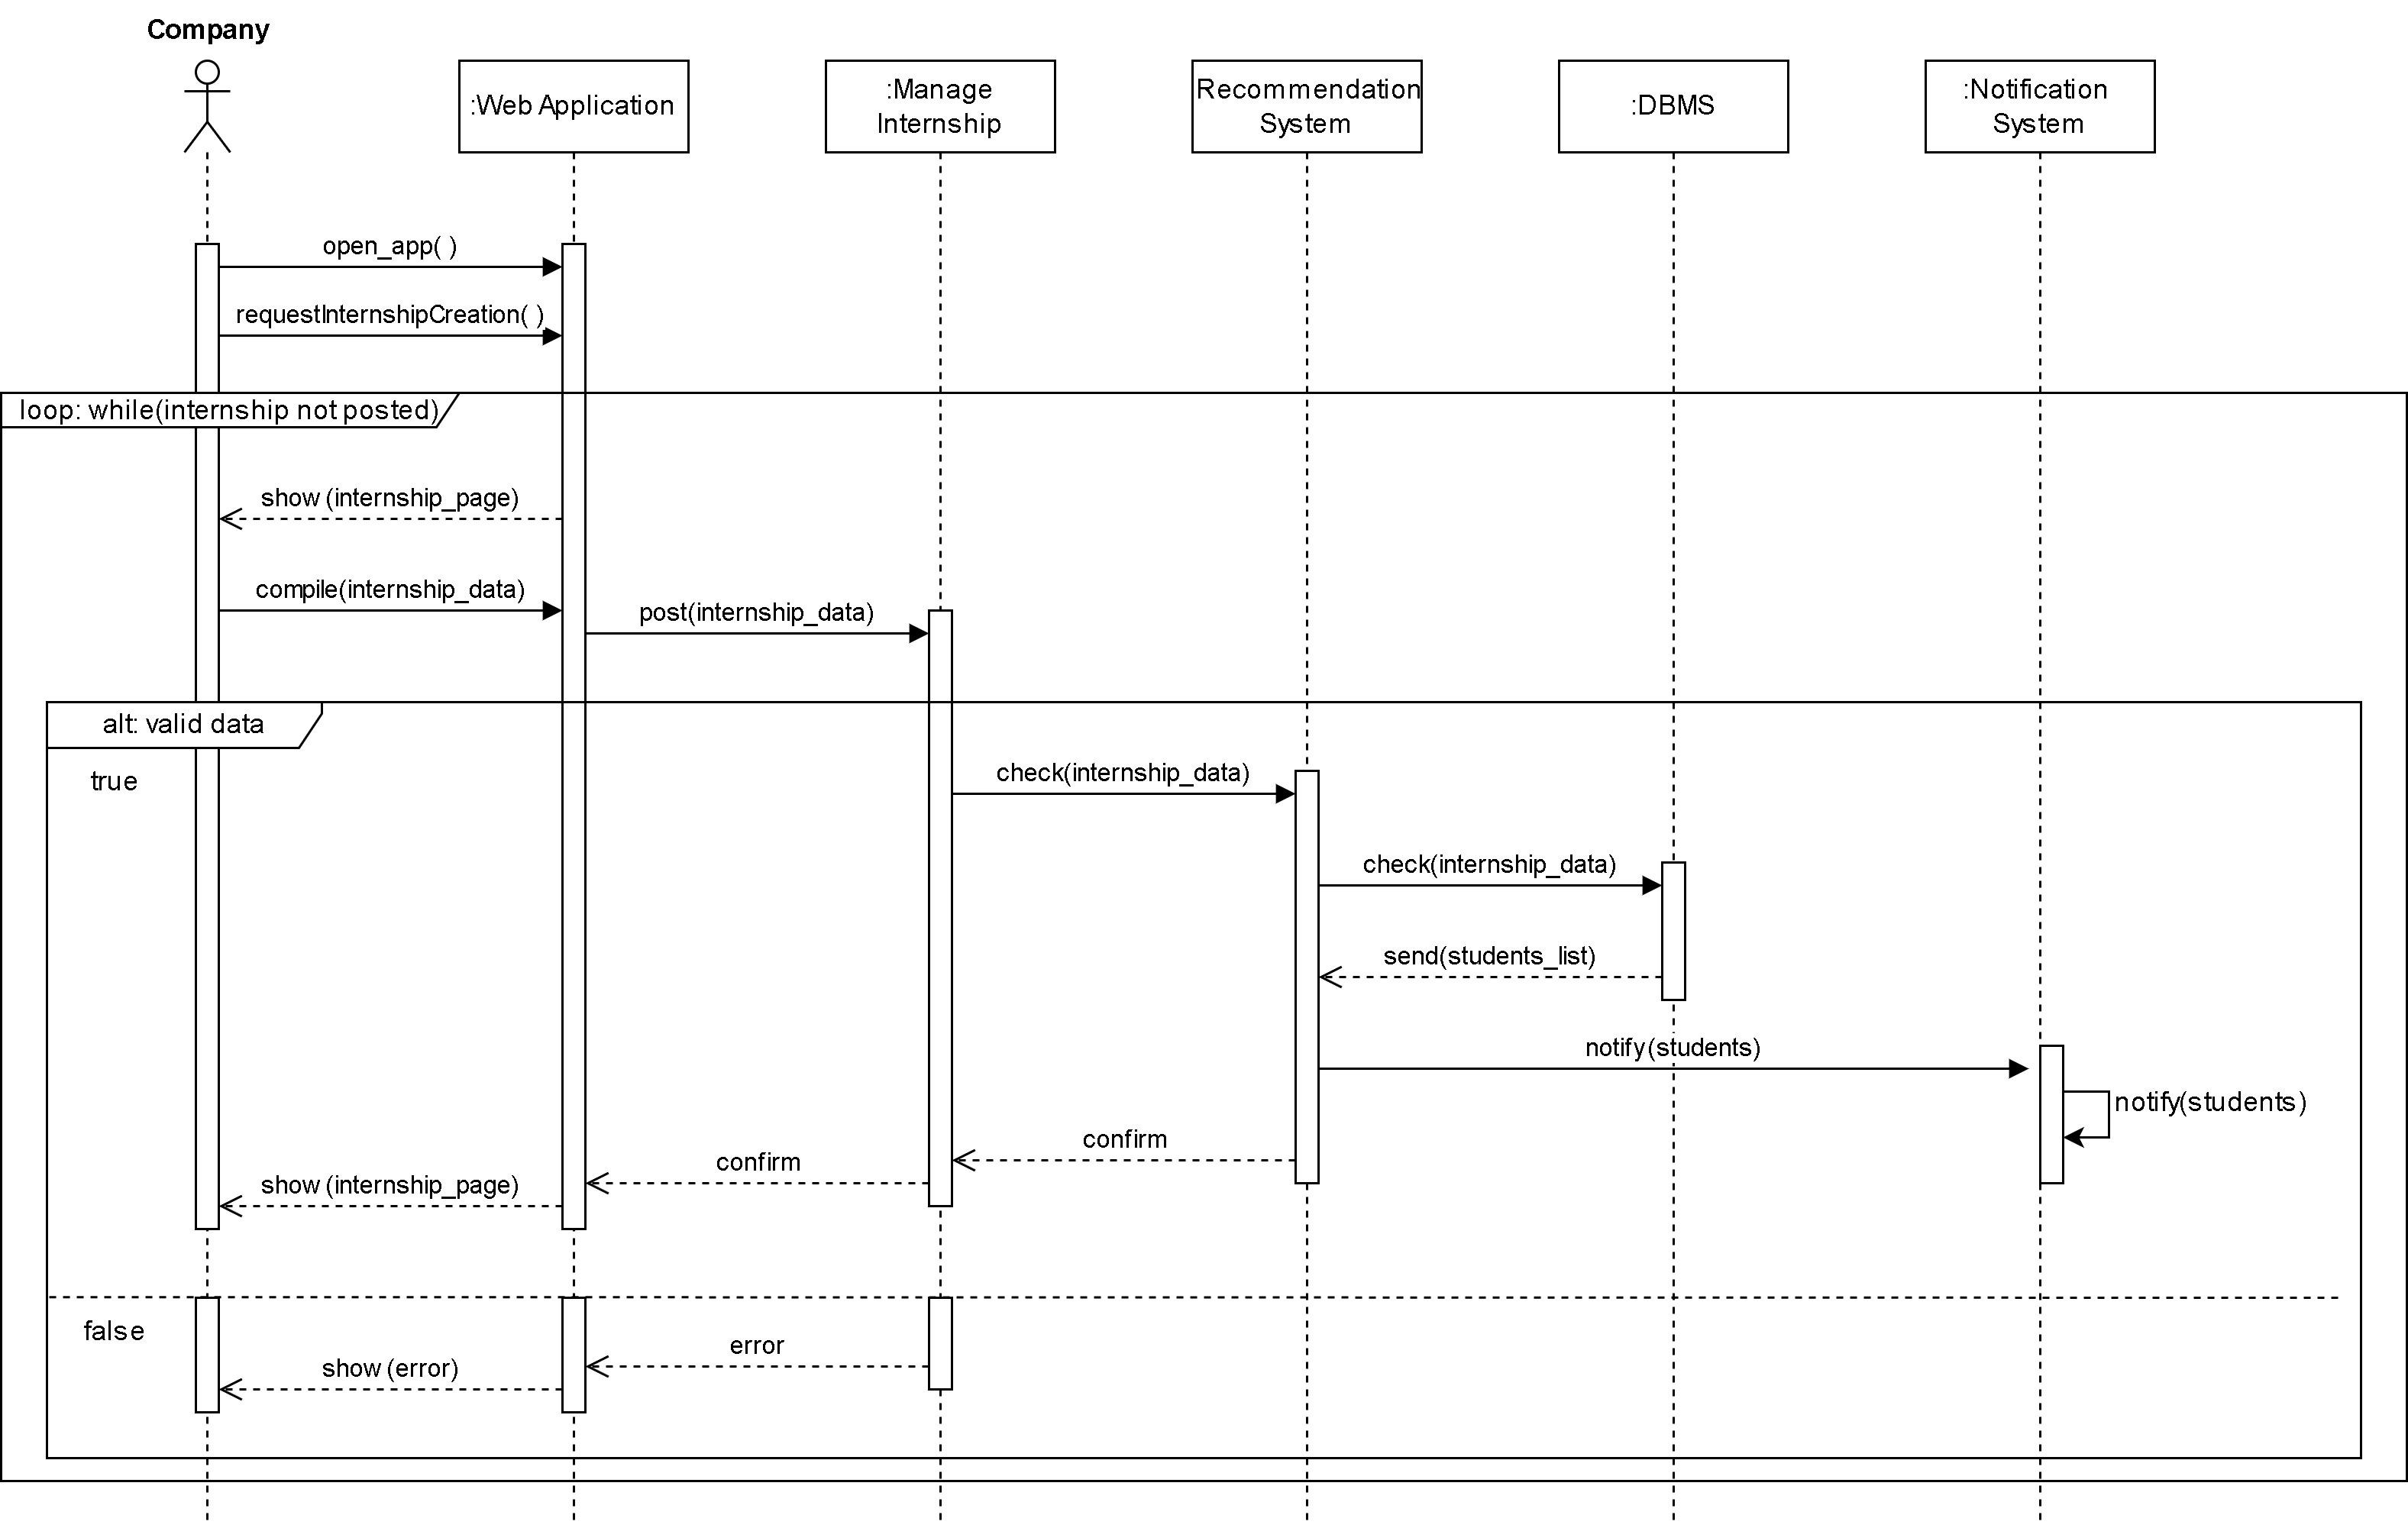
\includegraphics[width=0.95\textwidth]{Images/Seq3}
\caption{Internship creation sequence diagram}\label{Seq3}
\end{figure}

\newpage

		\subsubsection{Internship application}
In the internship application process, the student interacts with the \textit{Web Application} to search for a specific internship and apply for it. The student searches for specific keywords in the search bar, which activates the \textit{Manage Internship module} and through the \textit{DBMS} it retrieves the correct internships. The results are show on the \textit{Web Application} and the student can apply for the ones that he prefers. When applying to the internship the \textit{Manage Internship} module interacts with the \textit{Notification System} to notify the company of the candidates.

\begin{figure}[H]
\centering
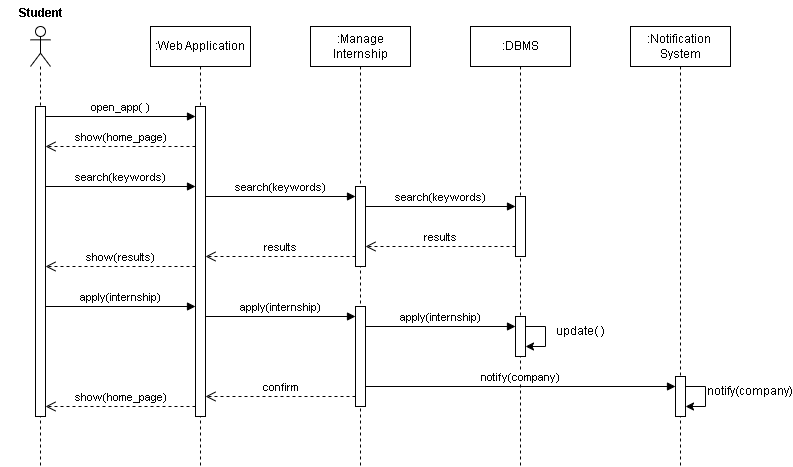
\includegraphics[width=0.95\textwidth]{Images/Seq4}
\caption{Internship application sequence diagram}\label{Seq4}
\end{figure}

\newpage

		\subsubsection{Form assignment for internship}
In the form assignment process, a company interacts with the \textit{Web Application} to assign a form to an already existing internship. In this case the \textit{Web Application} needs to interact with the \textit{Form Management} module to assign the form to the internship, and the \textit{Notification System} to notify all the candidates of the form to fill. Notice that this flow happens only when assigning a valid form, trying to assign an empty form shows an error message.
		
\begin{figure}[H]
\centering
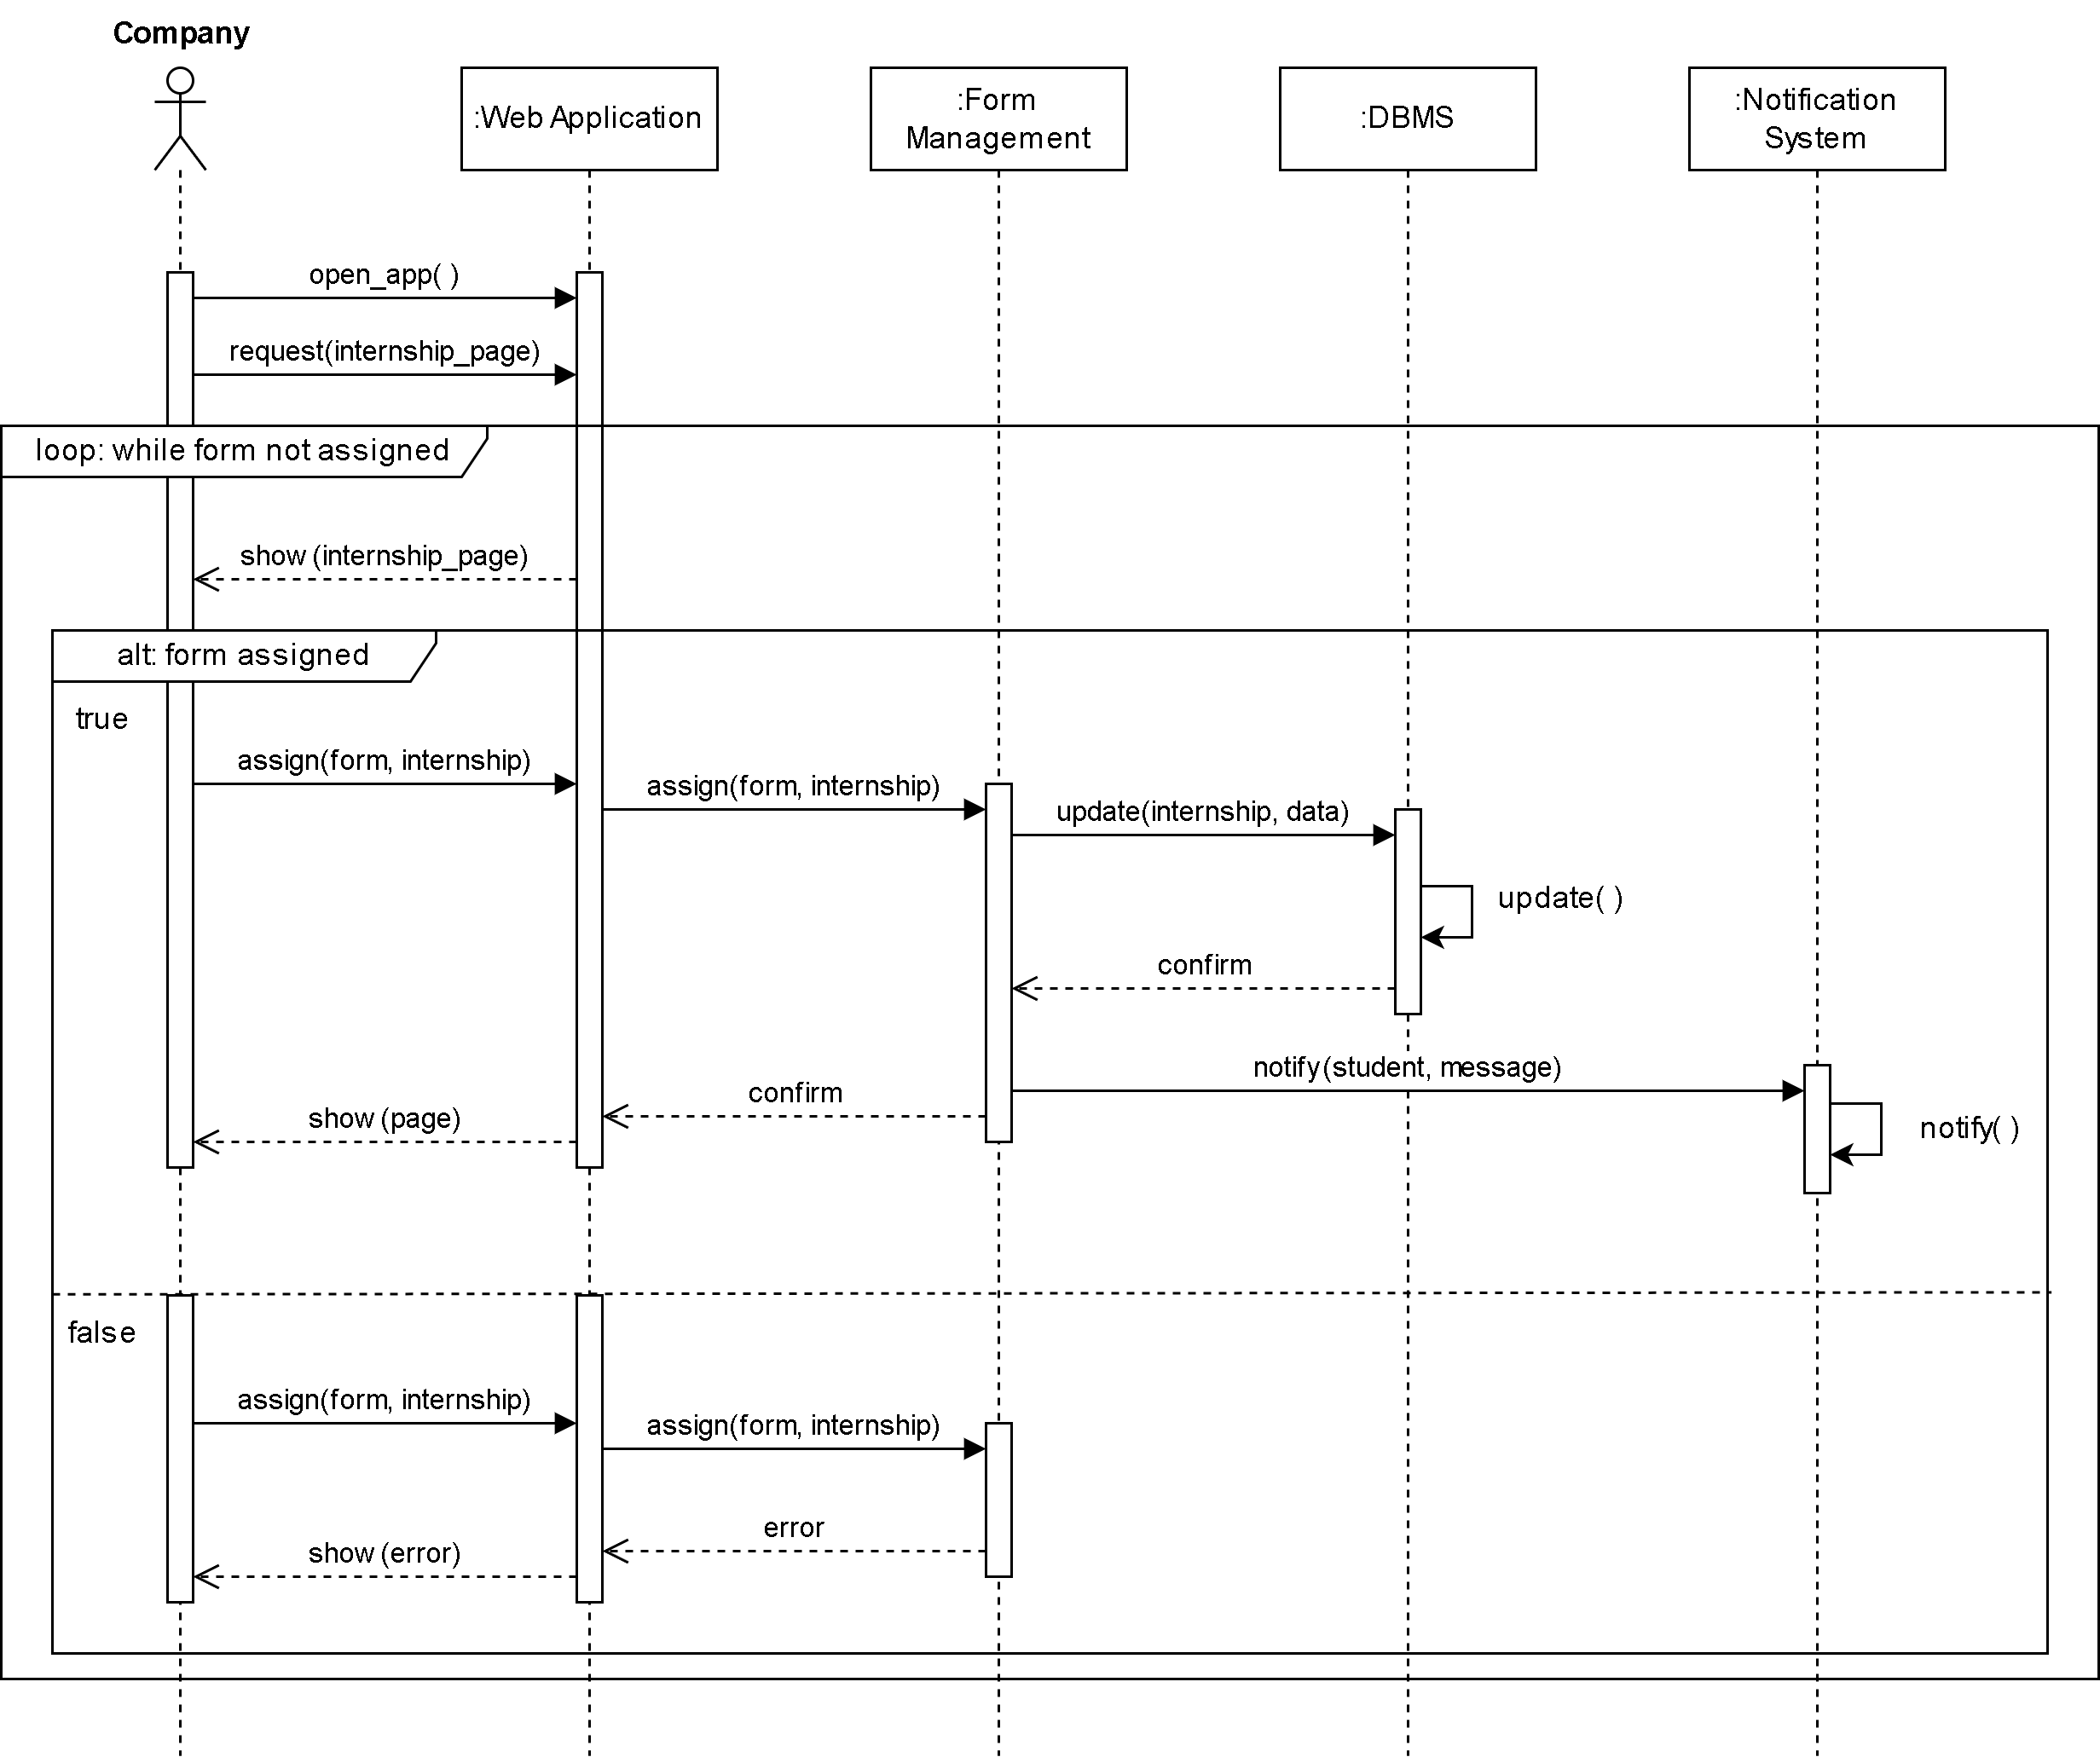
\includegraphics[width=0.95\textwidth]{Images/Seq5}
\caption{Form assignment sequence diagram}\label{Seq5}
\end{figure}

\newpage

		\subsubsection{Form compilation}
In the form compilation process, the student interacts with the \textit{Web Application} to fill and submit a form for an internship.	In this case the \textit{Web Application} needs to interact with the \textit{Form Management} module to save the answer in the data base, and the \textit{Notification System} to notify the company of the compiled forms they need to correct. Trying to submit an form with a missing answer will prevent the submission and show an error message instead.
		
\begin{figure}[H]
\centering
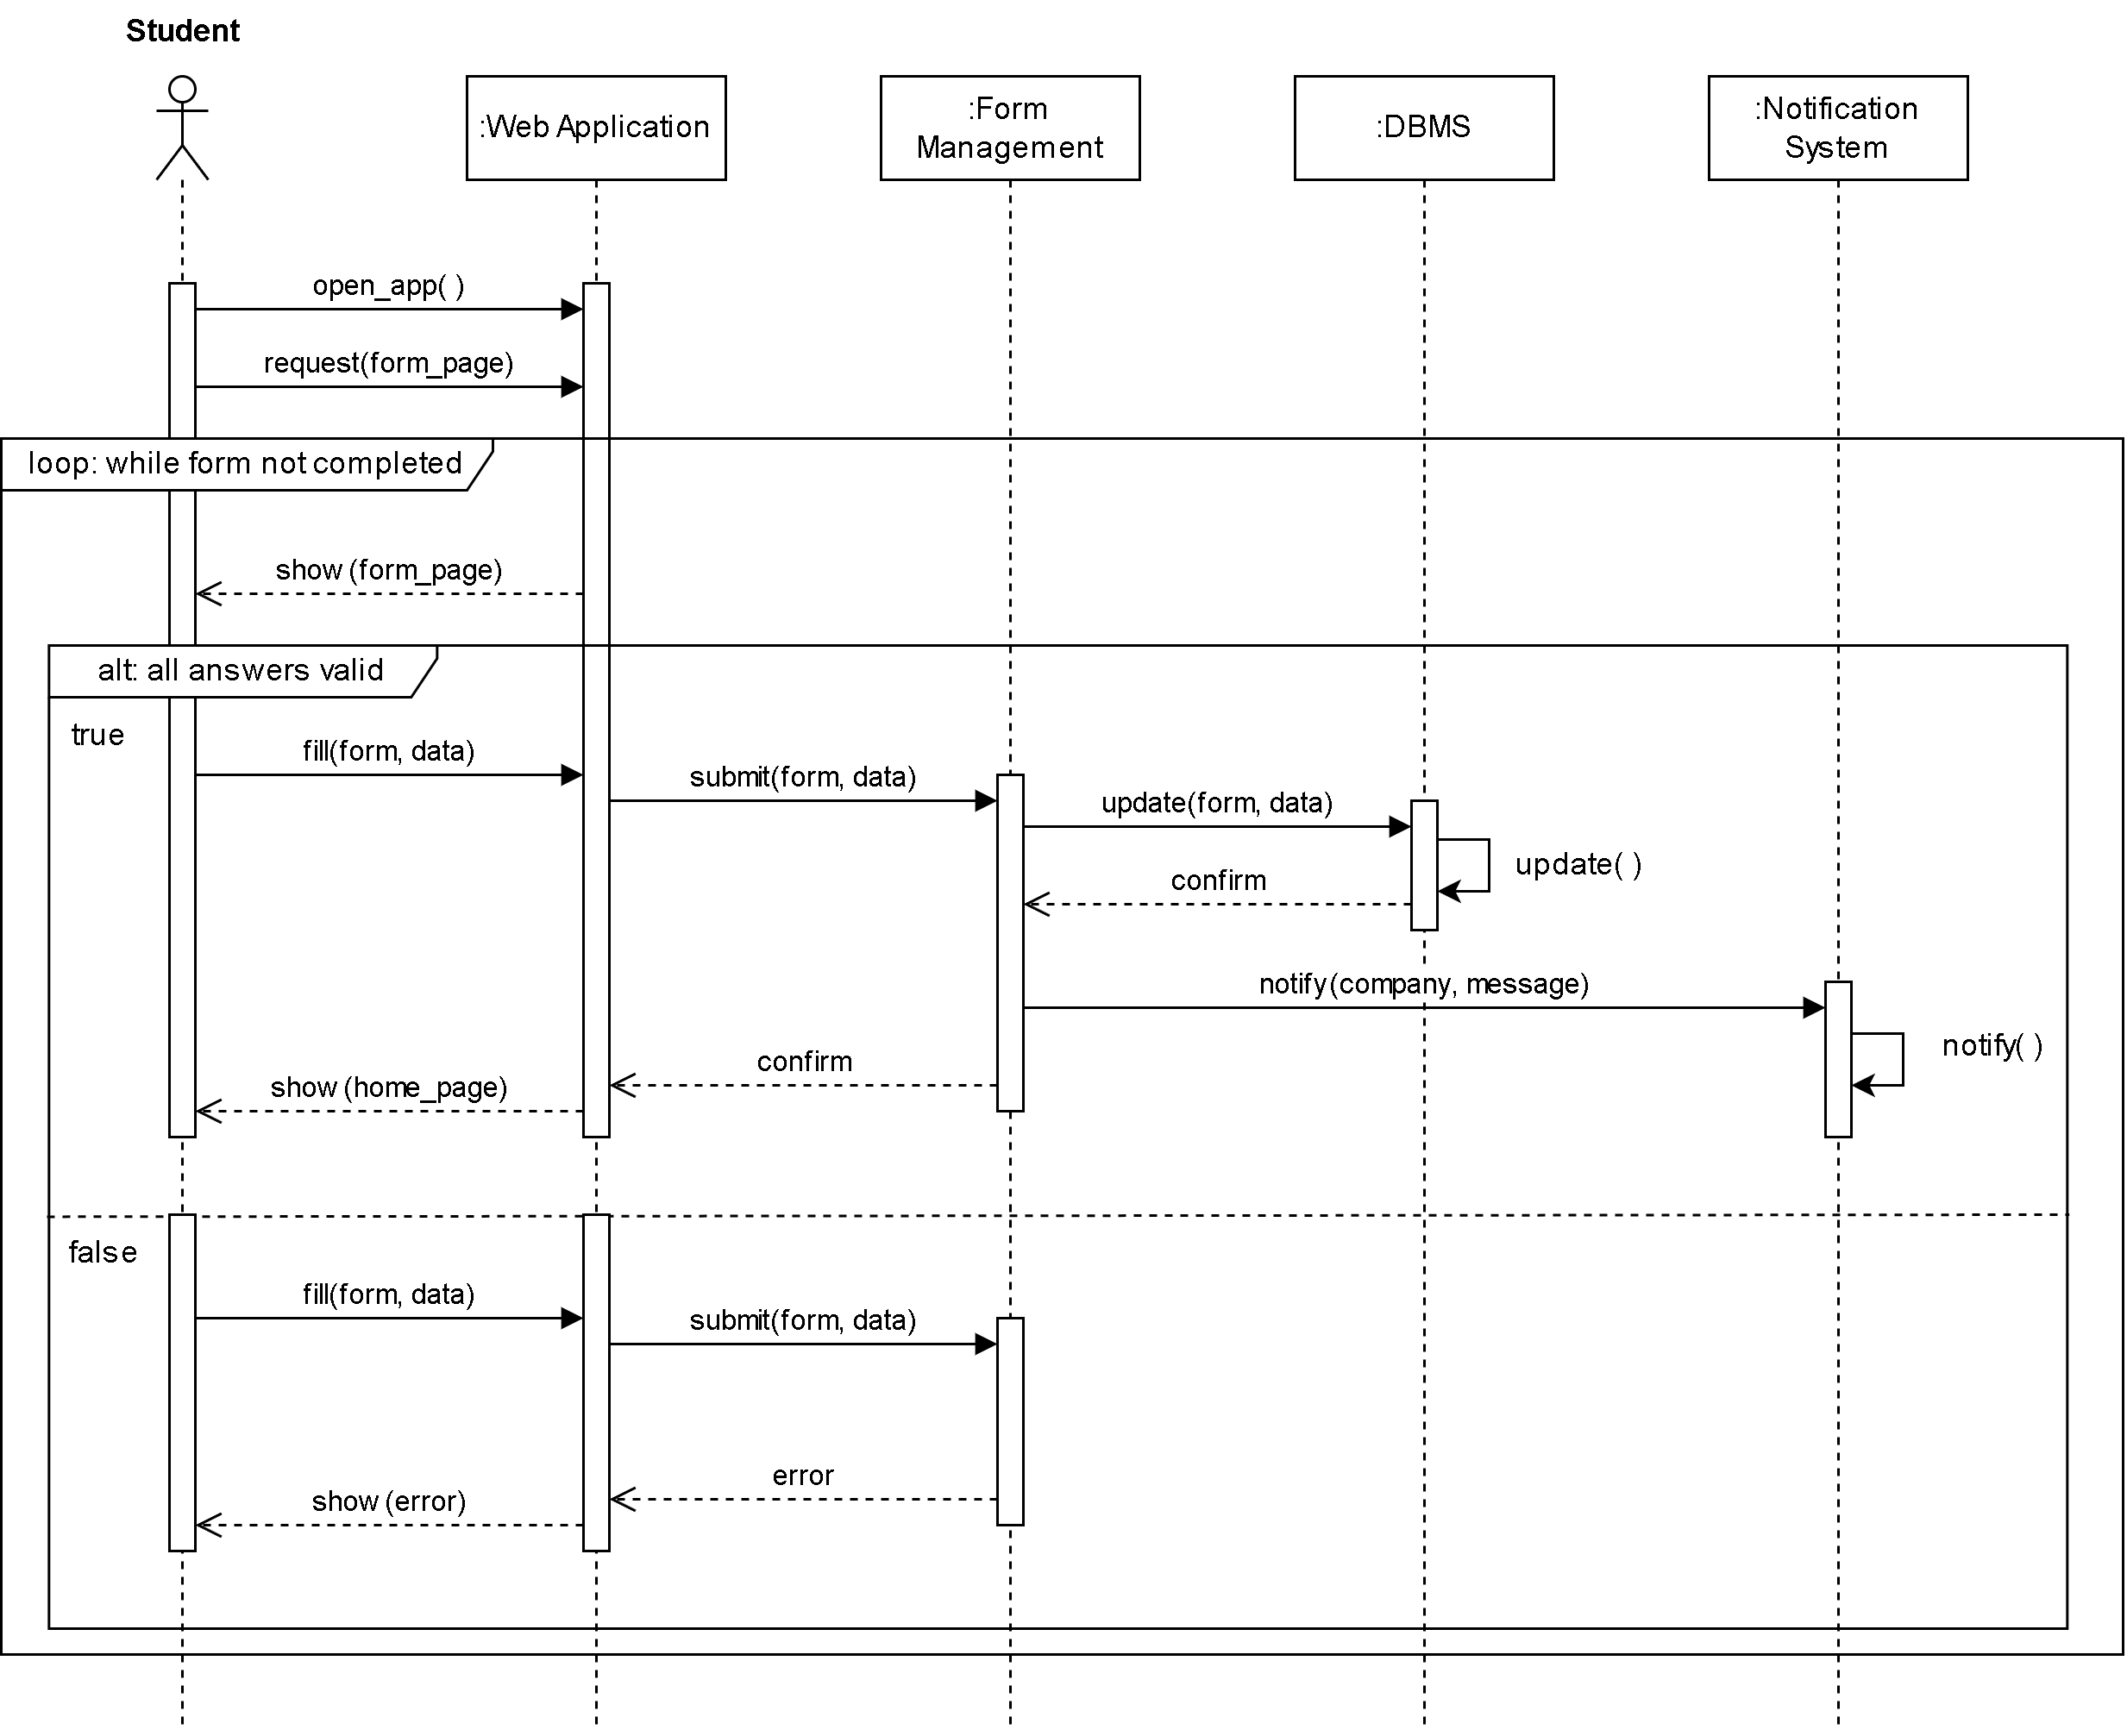
\includegraphics[width=0.95\textwidth]{Images/Seq6}
\caption{Form compilation sequence diagram}\label{Seq6}
\end{figure}

\newpage

		\subsubsection{Form correction}
In the form correction process a company interacts with the \textit{Web Application} to correct a form submitted by a student. In this case the \textit{Web Application} needs to interact with the \textit{Form Management} module to save the score of the candidate for later use in the ranking system. The score can be submitted only when each individual question is given a valid score.

\begin{figure}[H]
\centering
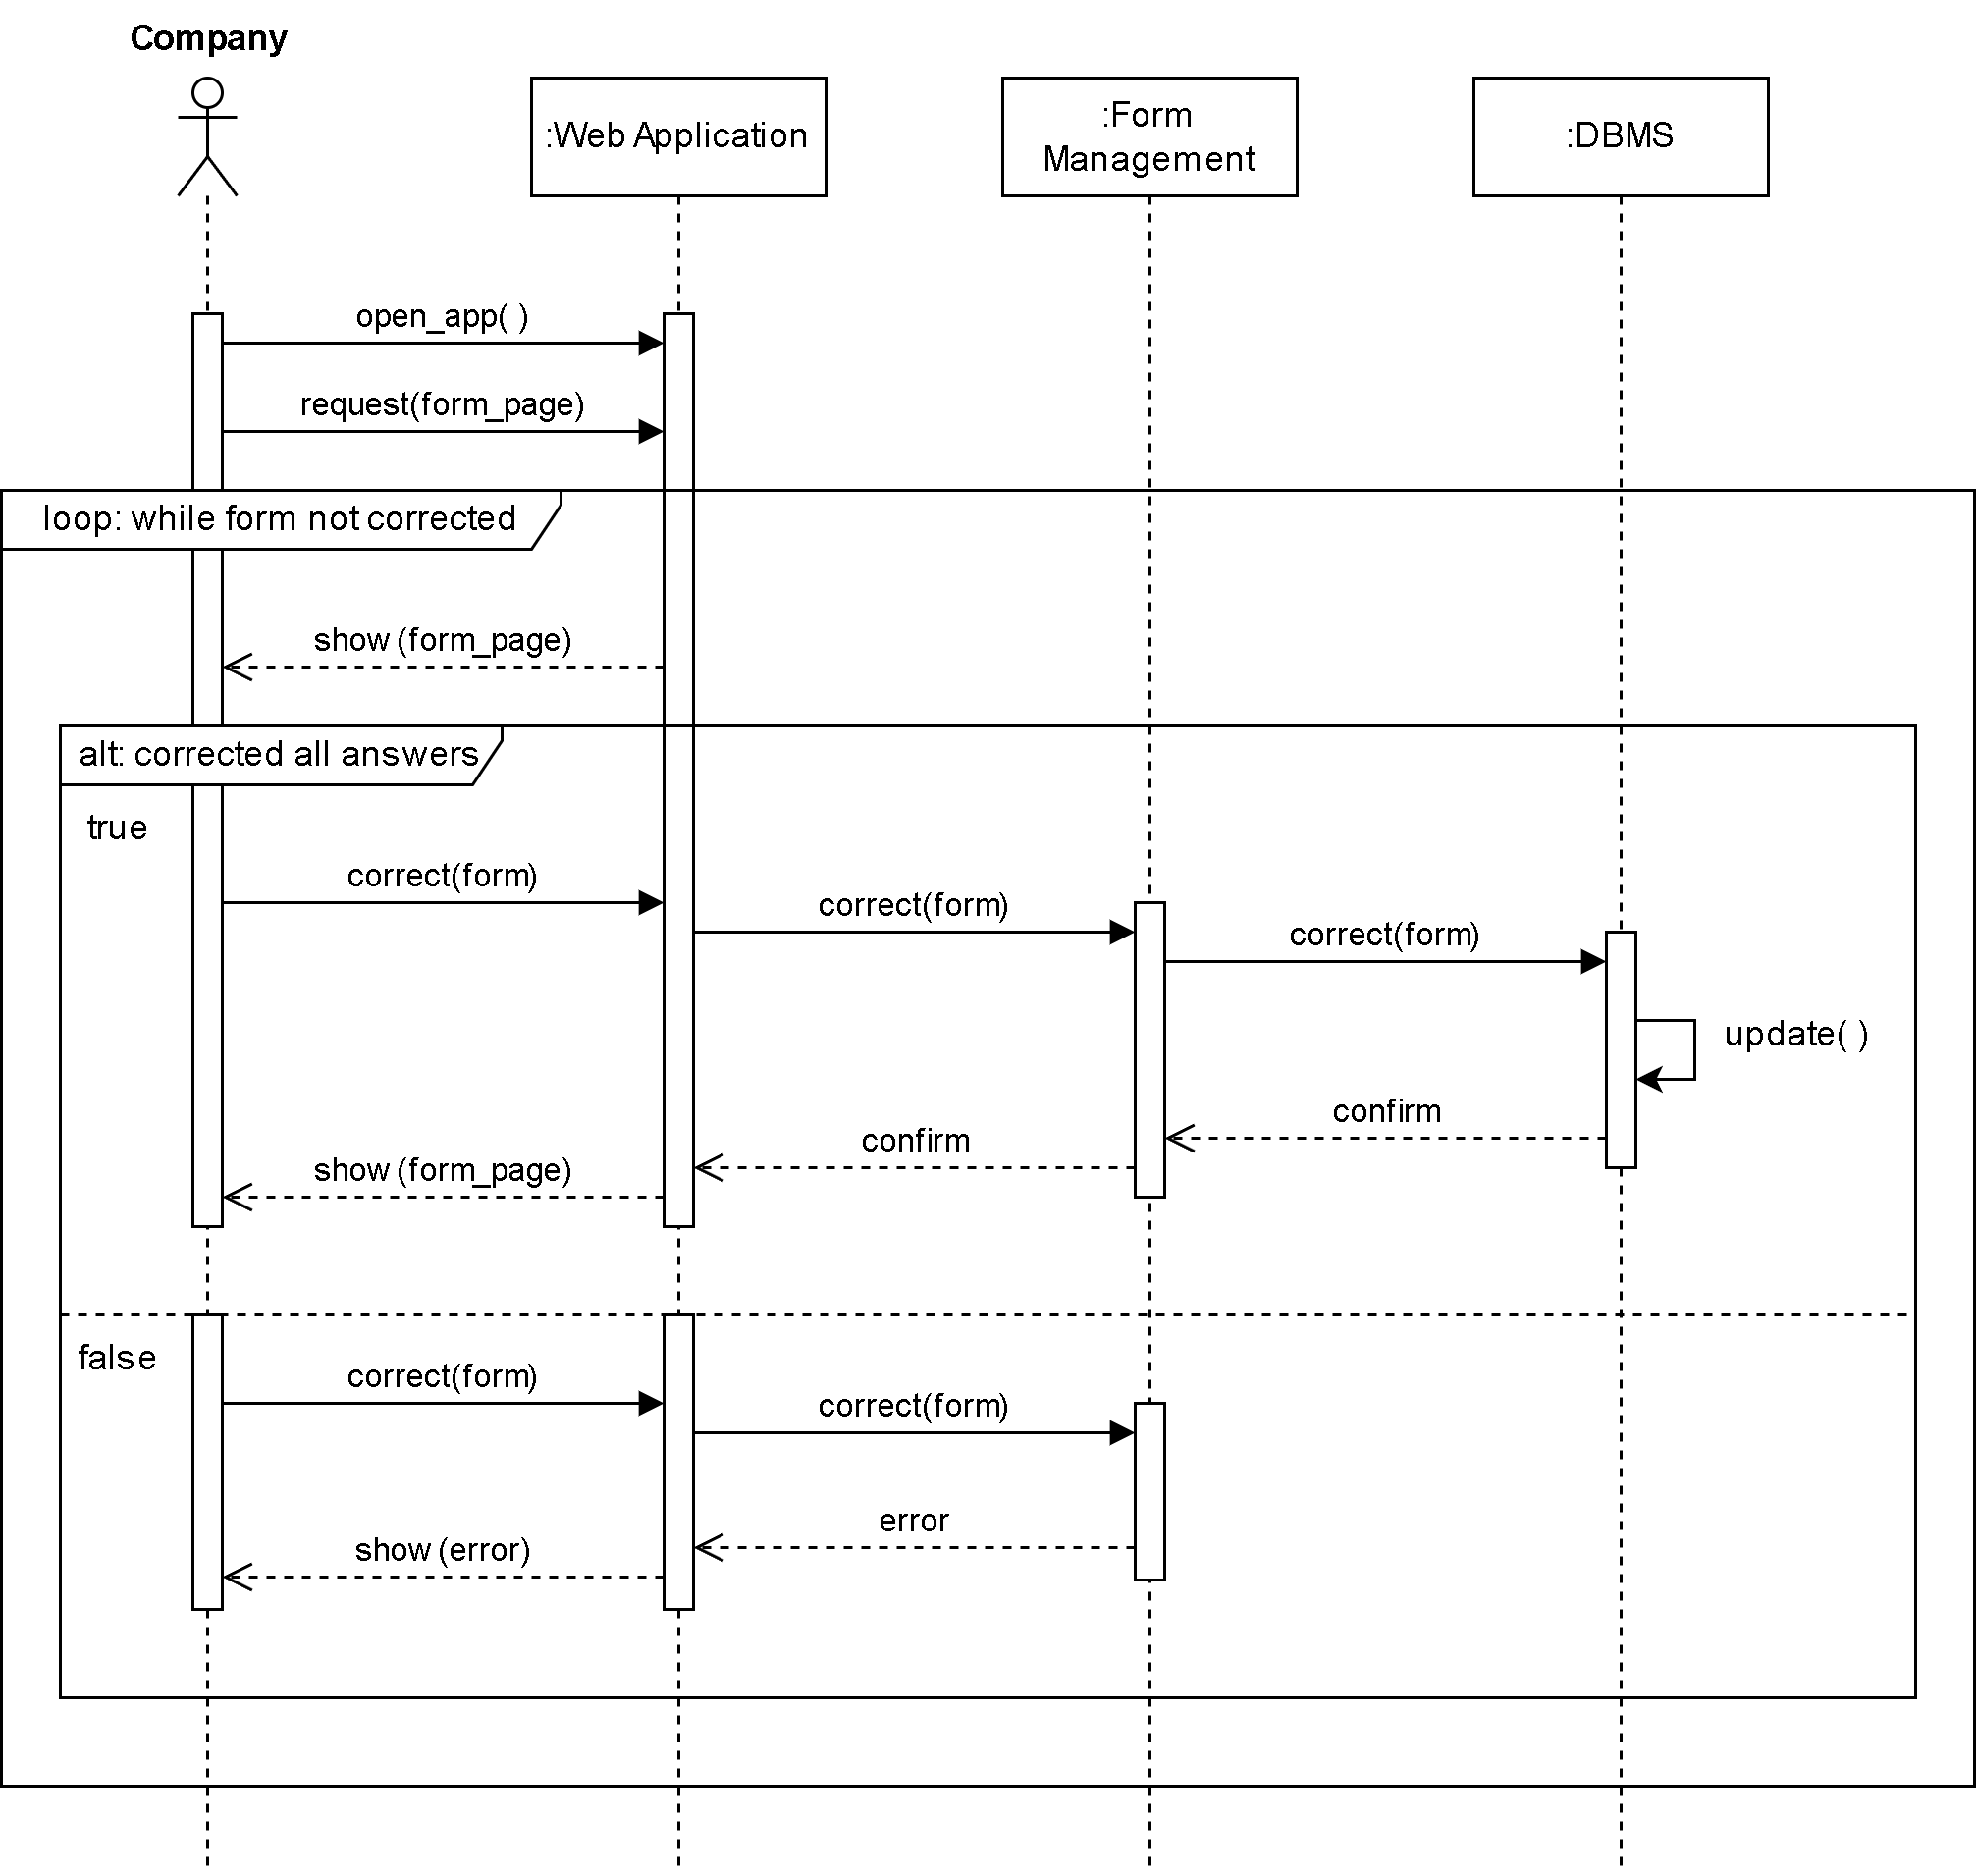
\includegraphics[width=0.95\textwidth]{Images/Seq7}
\caption{Form correction sequence diagram}\label{Seq7}
\end{figure}

\newpage

		\subsubsection{Student selection}
In the student selection process a company interacts with the \textit{Web Application} to select the candidates that can move to the next phase of the selection process or that were chosen to participate in the actual internship. In this case the \textit{Web Application} needs to interact with the \textit{Internship Selection} module and the \textit{Ranking System} to retrieve from the data base the scores of all the candidates and format the in a readable way. The ranking is shown on the screen of the company application, and they can then choose a list of students that will advance to next phase. For this reason the \textit{Internship Selection} module needs to also interact with the \textit{Notification System}.

\begin{figure}[H]
\centering
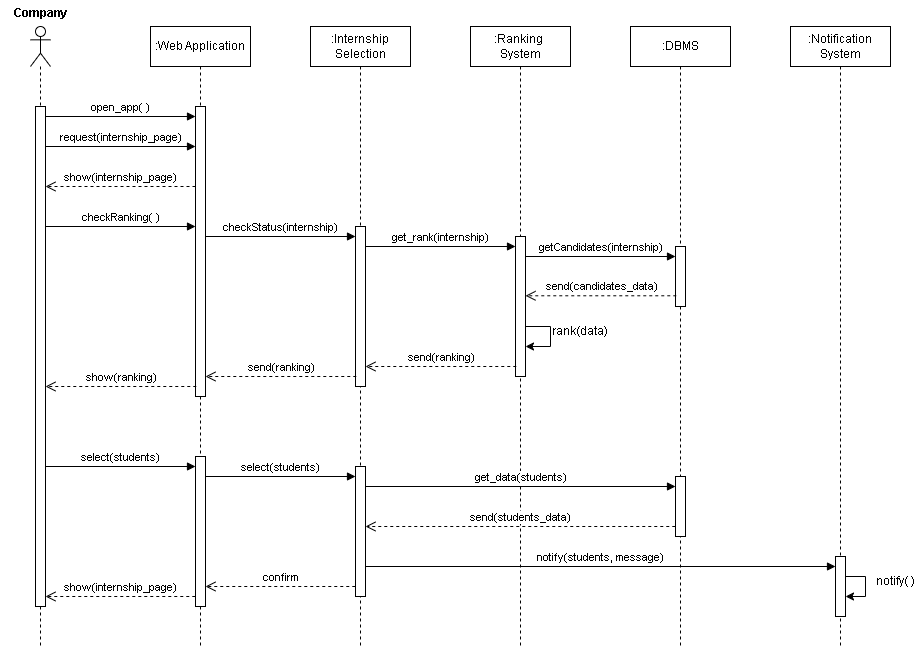
\includegraphics[width=0.95\textwidth]{Images/Seq8}
\caption{Student selection sequence diagram}\label{Seq8}
\end{figure}

\newpage
	
	\subsection{Component interfaces}
\begin{figure}[H]
\centering
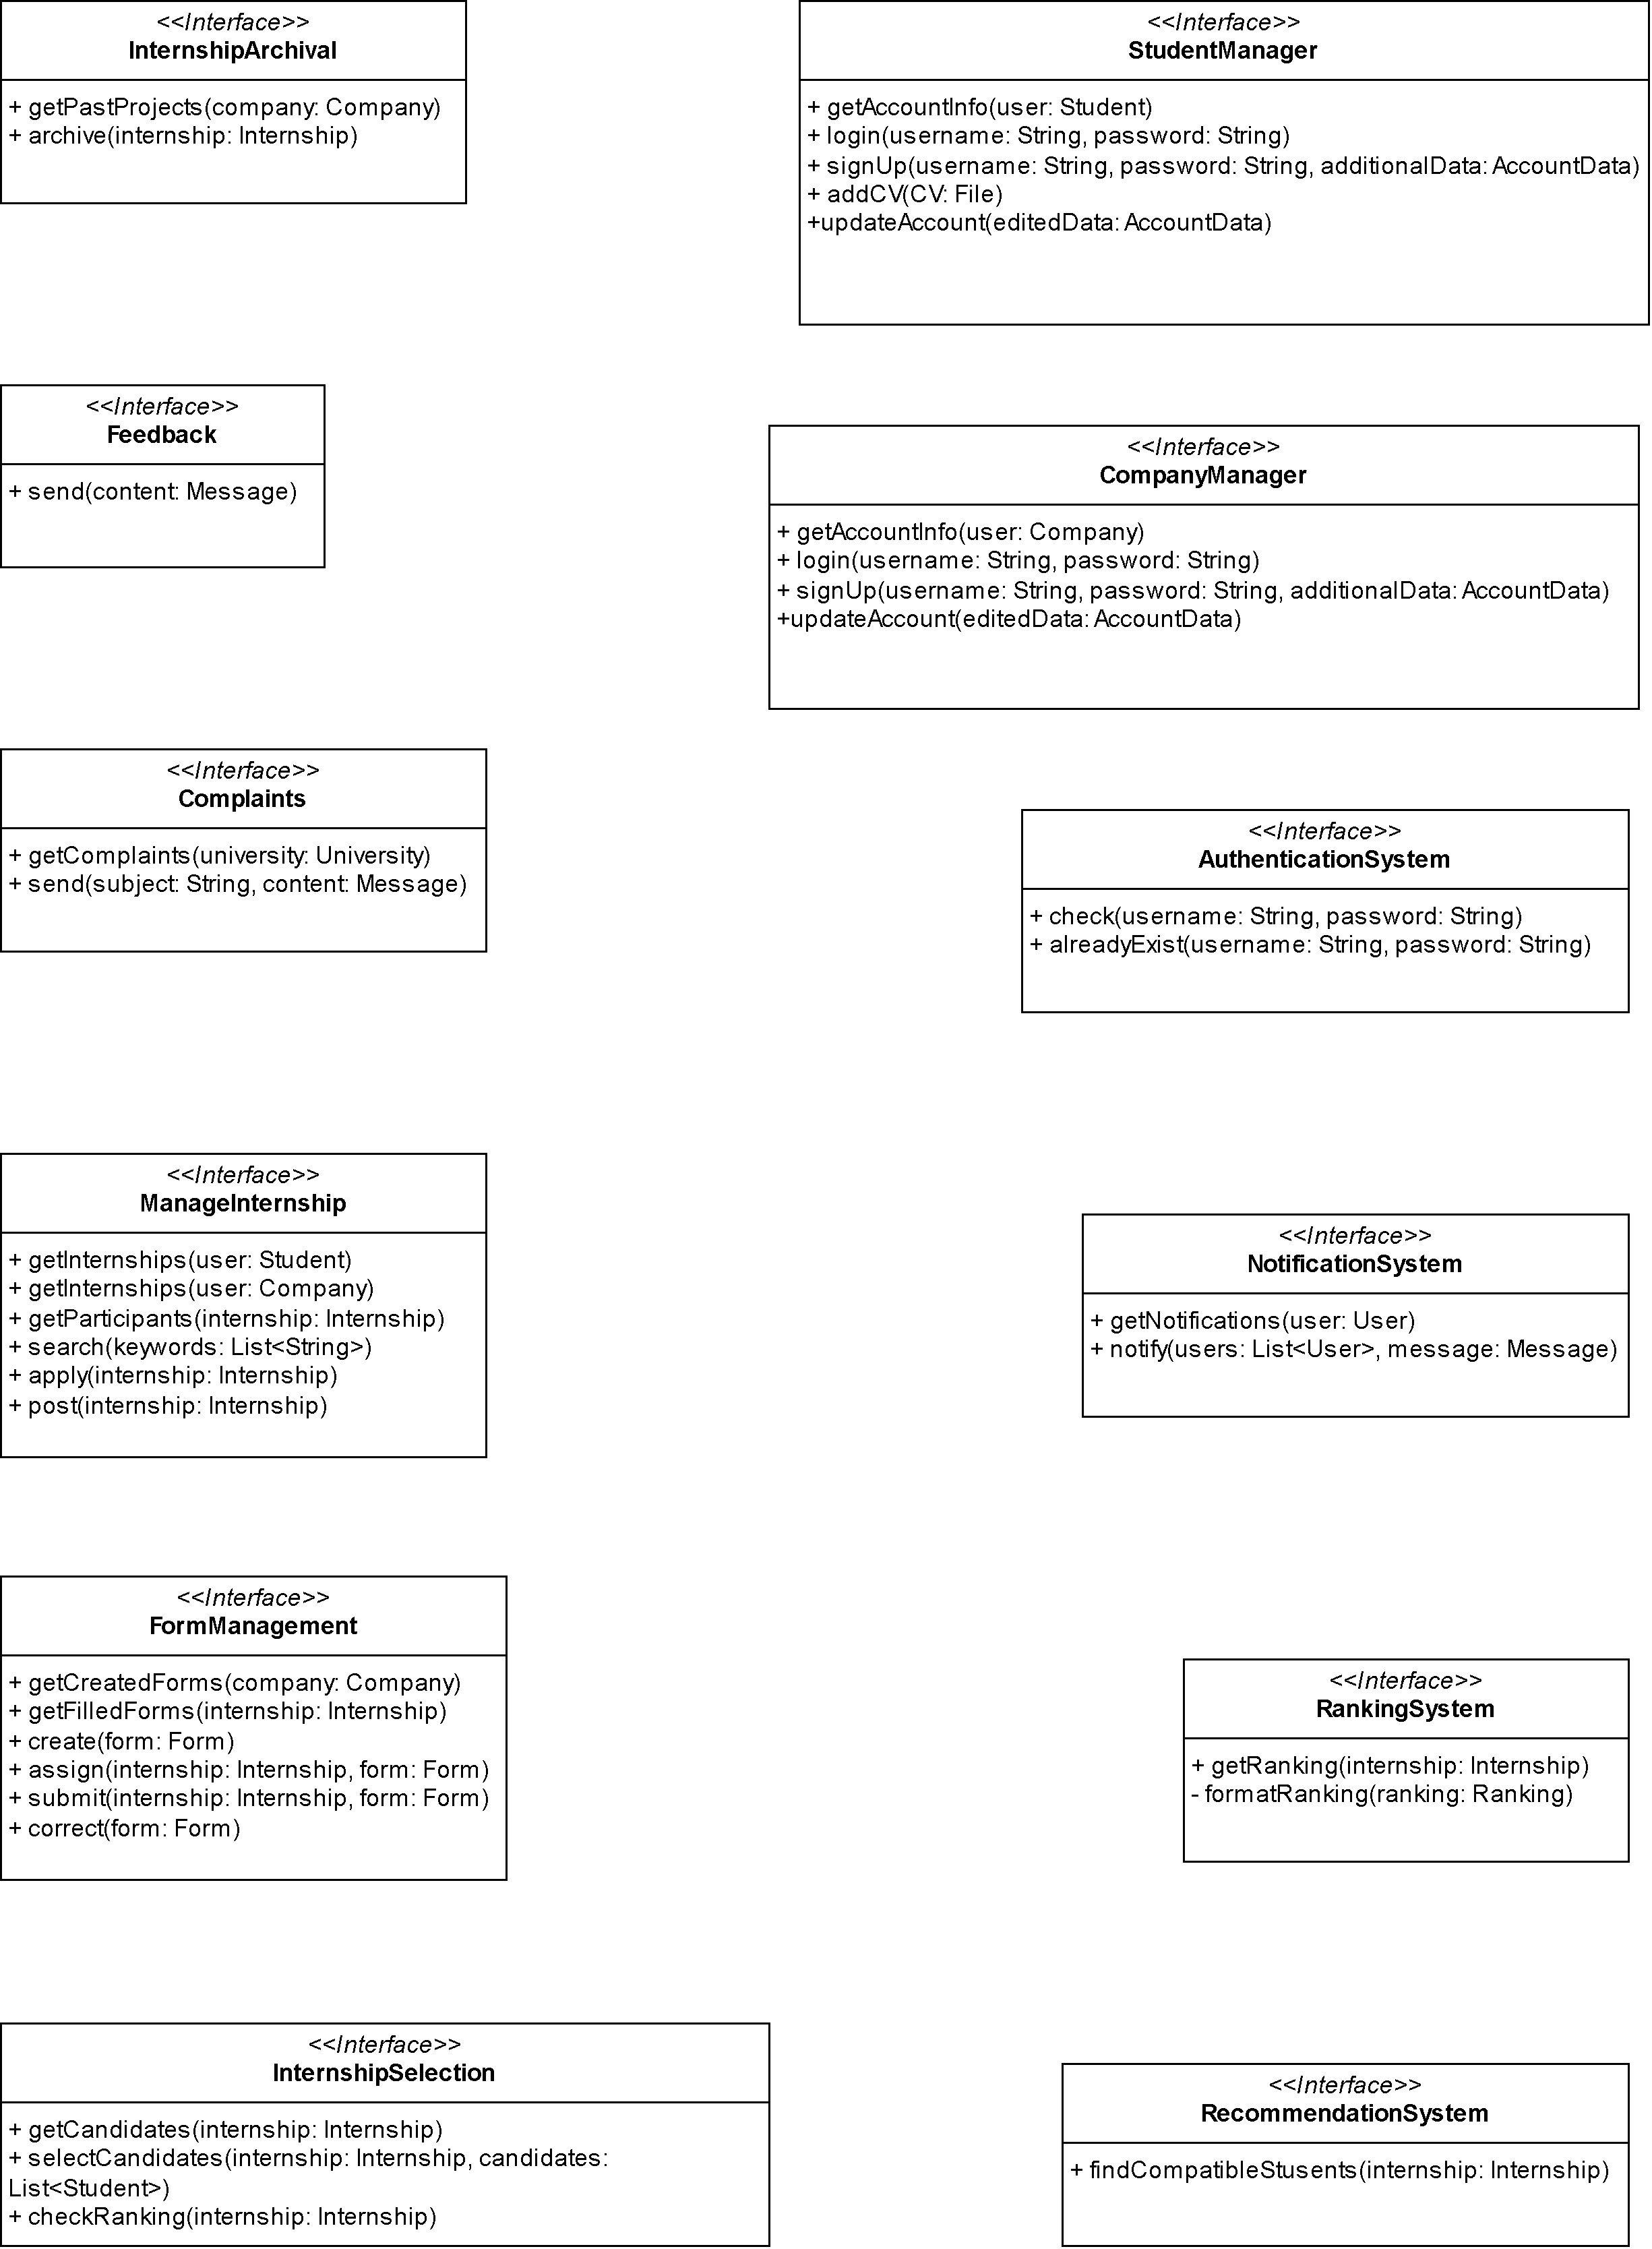
\includegraphics[width=0.98\textwidth]{Images/CompInterface}
\caption{Component interfaces diagram}\label{CompInterface}
\end{figure}

\newpage	

In figure [\ref{CompInterface}] we can see a list of all the interfaces and their respective exposed methods. In this section we are going to provide a more detailed description of such interfaces.
\begin{itemize}
\item \textbf{Internship Archival}:
	\begin{itemize}
	\item \textit{getPastProjects()}: Allows a user to retrieve all past projects of a given company.
	\item \textit{archive()}: Allows a company to add a concluded internship to their list of past projects.
	\end{itemize}
	
\item \textbf{Feedback}:
	\begin{itemize}
	\item \textit{send()}: Allows a user to send a feedback to the developers.
	\end{itemize}
	
\item \textbf{Complaints}:
	\begin{itemize}
	\item \textit{getComplaints()}: Allows a university to retrieve all complaints that involve at least one of their student.
	\item \textit{send()}: Allows a user to file a complaint.
	\end{itemize}
	
\item \textbf{Manage Internship}:
	\begin{itemize}
	\item \textit{getInternships()}: Overload parameters
		\begin{itemize}
		\item Student: Allows a student to retrieve all the internship to show in his home page.
		\item Company: Allows a user to retrieve all the internships that have been created by a certain company.
		\end{itemize}
	\item \textit{getParticipats()}: Allows a company to retrieve all the candidates of an internship.
	\item \textit{search()}: Allows a student to retrieve all internships compatible with a list of keywords.
	\item \textit{apply()}: Allows a student to apply for a specific internship.
	\item \textit{post()}: Allows a company to post regarding a newly created internship.
	\end{itemize}
	
\item \textbf{Form Management}:
	\begin{itemize}
	\item \textit{getCreatedForms()}: Allows a company to retrieve all form they created.
	\item \textit{getFilledForms()}: Allows a company to retrieve all forms that have been filled for a specific internship.
	\item \textit{create()}: Allows a company to save the form they created.
	\item \textit{assign()}: Allows a company to send all the candidates of an internship the form for the first selection phase.
	\item \textit{submit()}: Allows a student to submit a form regarding a specific internship.
	\item \textit{correct()}: Allows a company to save the score of a corrected form.
	\end{itemize}
	
\item \textbf{Internship Selection}:
	\begin{itemize}
	\item \textit{getCandidates()}: Allows a company to retrieve all the available candidates that want to participate in a given internship.
	\item \textit{selectCandidates()}: Allows a company to select a list of candidates, allowing them to move on to the next selection phase.
	\item \textit{checkRanking()}: Allows a company to retrieve the ranking for the current selection phase of a given internship.
	\end{itemize}
	
\item \textbf{Student Manager}:
	\begin{itemize}
	\item \textit{getaccountInfo()}: Allows a student to retrieve all the required information to show the profile page.
	\item \textit{login()}: Allows a student to try logging in his account using the given username and password.
	\item \textit{signUp()}: Allows a student to try creating a new account with the specified information.
	\item \textit{addCV()}: Allows a student to add a file in the CV section.
	\item \textit{update()}: Allows a student to edit the personal information shown in the profile.
	\end{itemize}
	
\item \textbf{Company Manager}:
	\begin{itemize}
	\item \textit{getaccountInfo()}: Allows a company to retrieve all the required information to show the profile page.
	\item \textit{login()}: Allows a company to try logging in his account using the given username and password.
	\item \textit{signUp()}: Allows a company to try creating a new account with the specified information.
	\item \textit{update()}: Allows a company to edit the personal information shown in the profile.
	\end{itemize}
\end{itemize}

The following modules contain methods that are called by the main modules, so the users cannot directly interact with them.

\begin{itemize}
\item \textbf{Authentication System}:
	\begin{itemize}
	\item \textit{check()}: Checks the correctness of the given credentials. This method is called by the \textit{login} method.
	\item \textit{alreadyExist()}: Checks if the given information already exist in the database. This method is called by the \textit{signUp} method.
	\end{itemize}
	
\item \textbf{Notification System}:
	\begin{itemize}
	\item \textit{getNotifications()}: Retrieves all the notifications to be shown to a specified user.
	\item \textit{notify()}: Sends a notification to a specified user.
	\end{itemize}
	
\item \textbf{Ranking System}:
	\begin{itemize}
	\item \textit{getRanking()}: Retrieves the ranking of a specified internship. This method is called by the \textit{checkRanking} method and returns the result of \textit{formatRanking}.
	\item \textit{formatRanking()}: Allows to format a ranking in a more readable way.
	\end{itemize}
	
\item \textbf{Recommendation System}:
	\begin{itemize}
	\item \textit{findCompatibleStudents()}: Retrieves all the compatible students for a given internship. This method is called by the \textit{post} method of Manage Internship.
	\end{itemize}
\end{itemize}
	
	\subsection{Selected architectural styles and patterns}
		\subsubsection{Architectural styles}
We already discussed about the tree-tier architecture with thin client approach and their benefits in the overview section (2.1).\\
Our choice in terms of communications protocol is HTTPS. First of all we chose it because it is one of the most used across most platforms, so it should not be too much of a problem to implement and second, is because it is the secure version of HTTP, the main protocol used to share data between a website and a browser. In addition HTTPS grants the security of the communication by encrypting the data to transfer. This is especially important in the case a user has to manage sensitive data regarding his profile.

		\subsubsection{Patterns}
\begin{itemize}
\item \textbf{Model-View-Controller (MVC)}: The logic in the application layer is structured using the MVC pattern, which allows the to organize the system in three different components:
	\begin{itemize}
	\item \textbf{Model}: Represents all the data logic in the system.
	\item \textbf{View}: Handles the presentation of the data to the user.
	\item \textbf{Controller}: Manages the interactions with the model.
	\end{itemize}
\item \textbf{Observer pattern}: Allows an object, named the subject, to maintain a list of dependent objects, called observers, and notify them whenever happens a change of state. This pattern is especially recommended given the use of the MVC pattern.
\item \textbf{Strategy pattern}: Allows the selection of an algorithm at runtime. Instead of implementing a single algorithm directly, the system receives runtime instructions as to which in a family of algorithms to use.
\item \textbf{Factory method}: Uses factory methods to deal with the problem of creating objects without having to specify their exact classes. The creation of an object is achieved by invoking a factory method, instead of calling a constructor.
\end{itemize}
	
	\subsection{Other design decisions}
\begin{itemize}
\item \textbf{OAuth 2.0}: OAuth 2.0, which stands for “Open Authorization”, is a standard designed to allow a website or application to access resources hosted by other web apps on behalf of a user. It provides consented access and restricts actions of what the client app can perform on resources on behalf of the user, without ever sharing the user's credentials.\\
\textbf{Important}: OAuth 2.0 is an authorization protocol and NOT an authentication protocol, which is why we have a custom \textit{Authentication System} module in the component view and not an authorization one.
\item \textbf{Notifications API}: Firebase Cloud Messaging (FCM), formerly known as Google Cloud Messaging (GCM), is a cross-platform push notification API for Android, iOS, and web applications. It is one of many tools under the Firebase platform umbrella, allowing you to combine various products for web and mobile production.\\
Since it's a Google product it is reliable and easy to implement thanks to a detailed documentation and several tutorials provided by the platform itself.
\end{itemize}

\newpage

\section{User interface design}
The aim of this section is to present the prototypes of the most important pages of the application and explain the features by emulating scenarios of a user interacting with the system.
\vspace{1\baselineskip} \\
\large{\textbf{Login and Sign Up page}}
\begin{figure}[H]
\centering
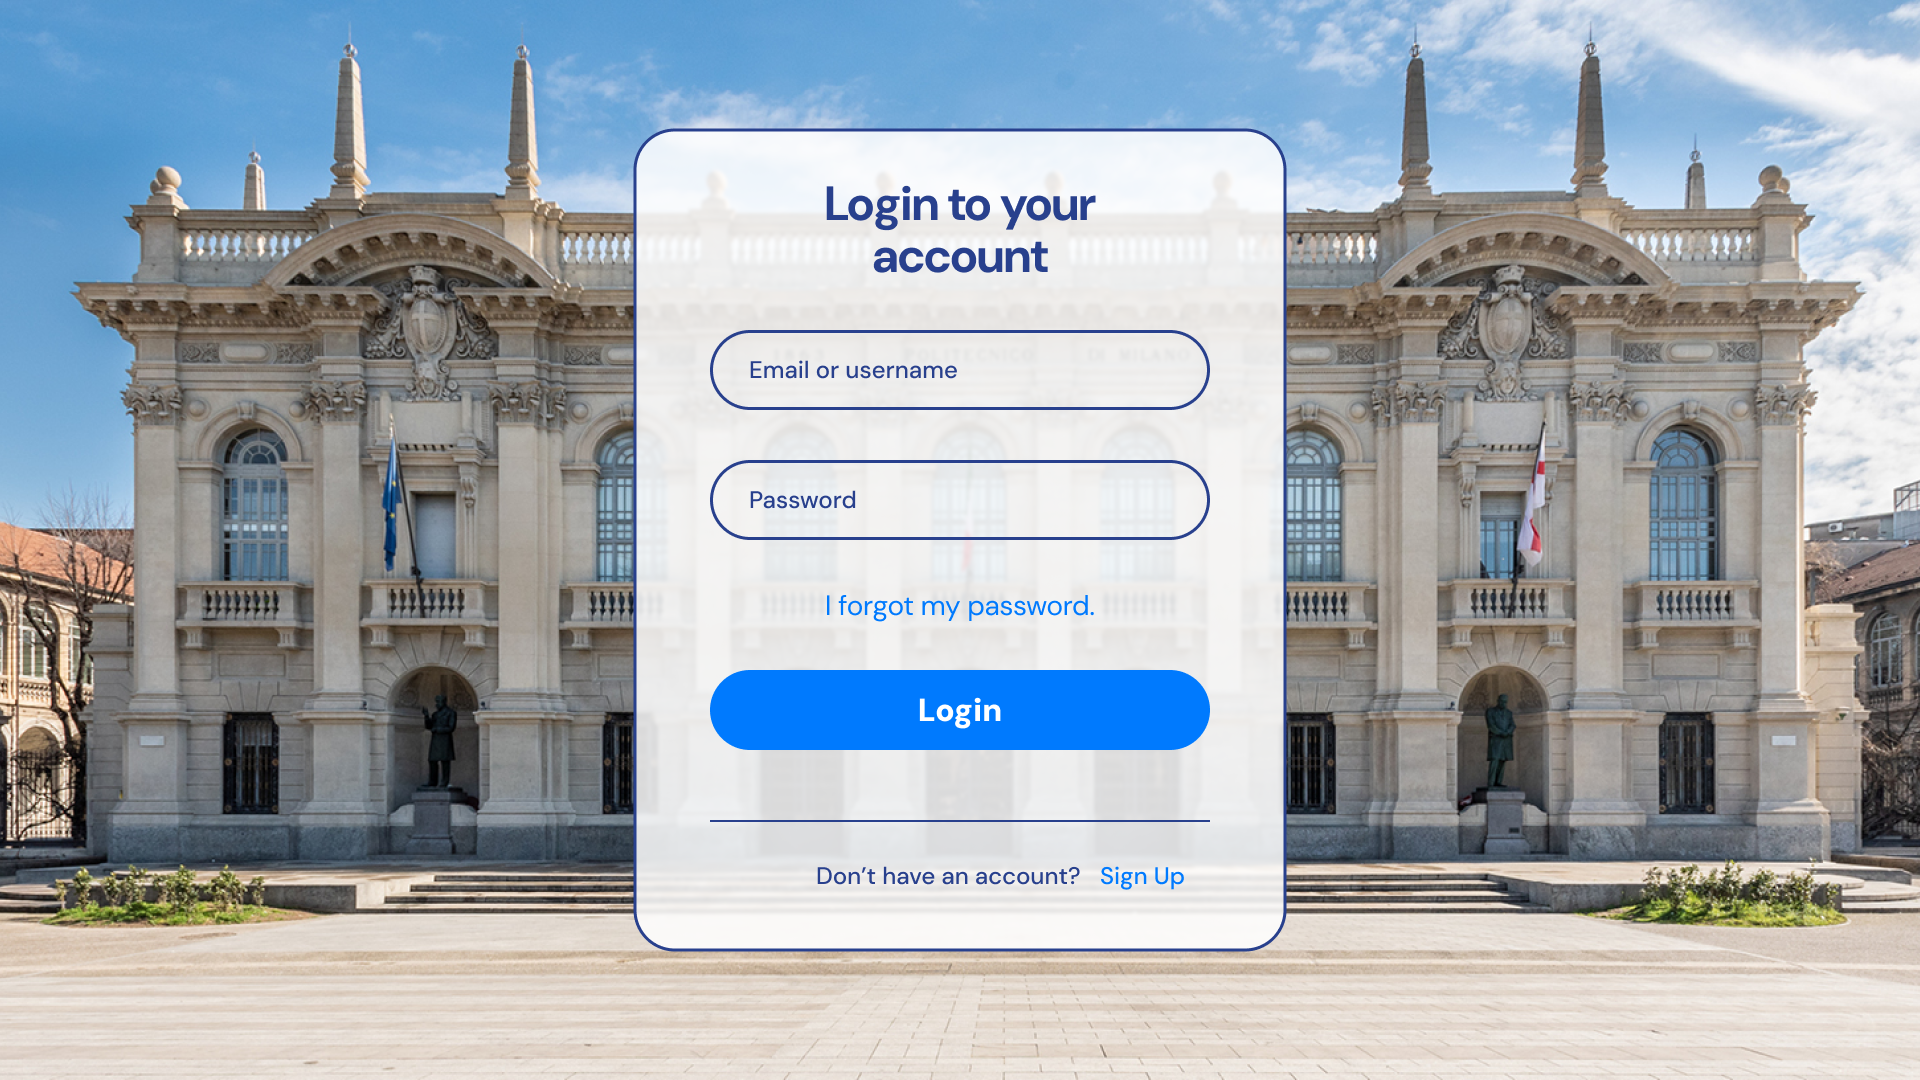
\includegraphics[width=0.98\textwidth]{Images/Login}
\caption{Login prototype page}\label{Login}
\end{figure}
\begin{figure}[H]
\centering
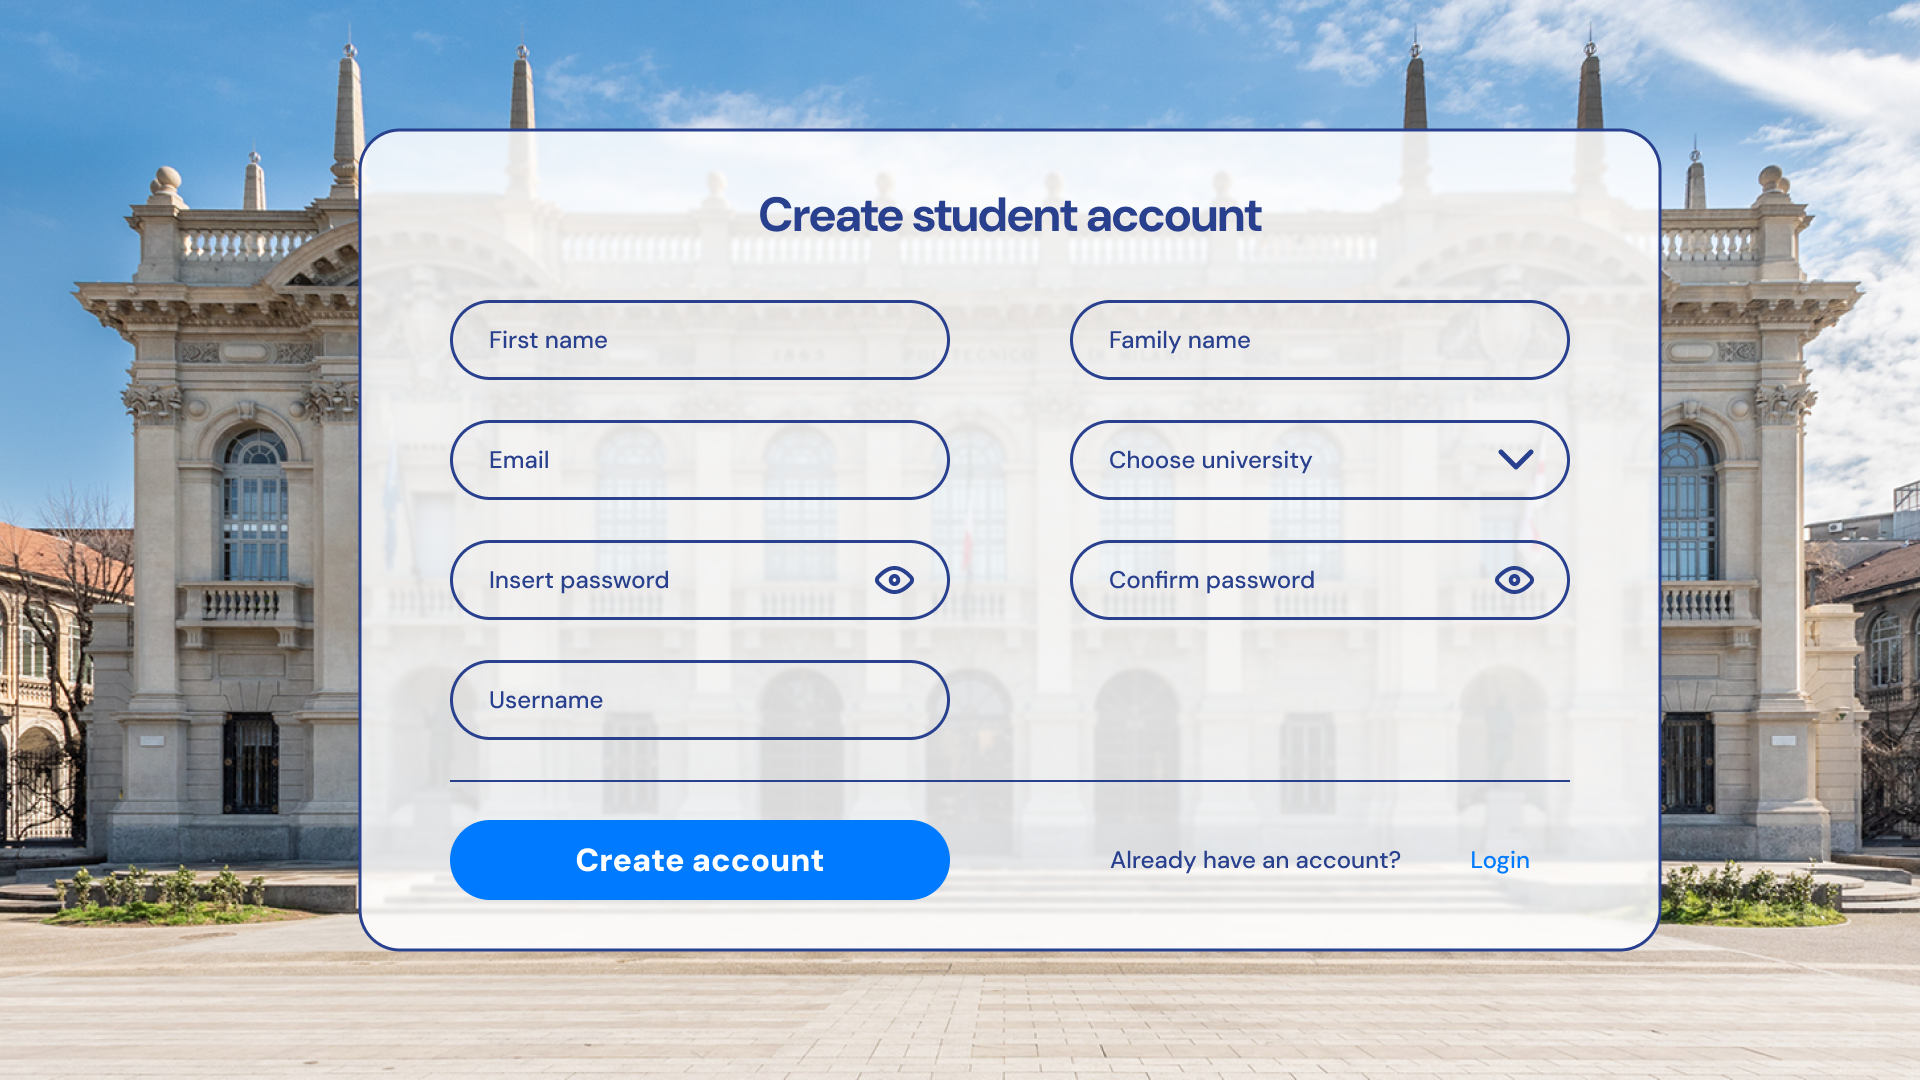
\includegraphics[width=0.98\textwidth]{Images/Sign Up}
\caption{Sign up prototype page}\label{Sign Up}
\end{figure}
\newpage
The picture [\ref{Login}] shows the prototype of the login page, allowing to either login by entering the correct credentials, create an account in case the user doesn't have one yet, or reset the password in case it was forgotten.\\
The picture [\ref{Sign Up}] shows the prototype of the sign up page for students, that allows students to create a new account by entering all the required information. In case the user already has an account there is a button that redirects to the login page. The case of a company creating an account is really similar to the one shown above with the simple difference that the user wont be required to choose a university.
\vspace{1\baselineskip} \\
\large{\textbf{Profile page}}
\begin{figure}[H]
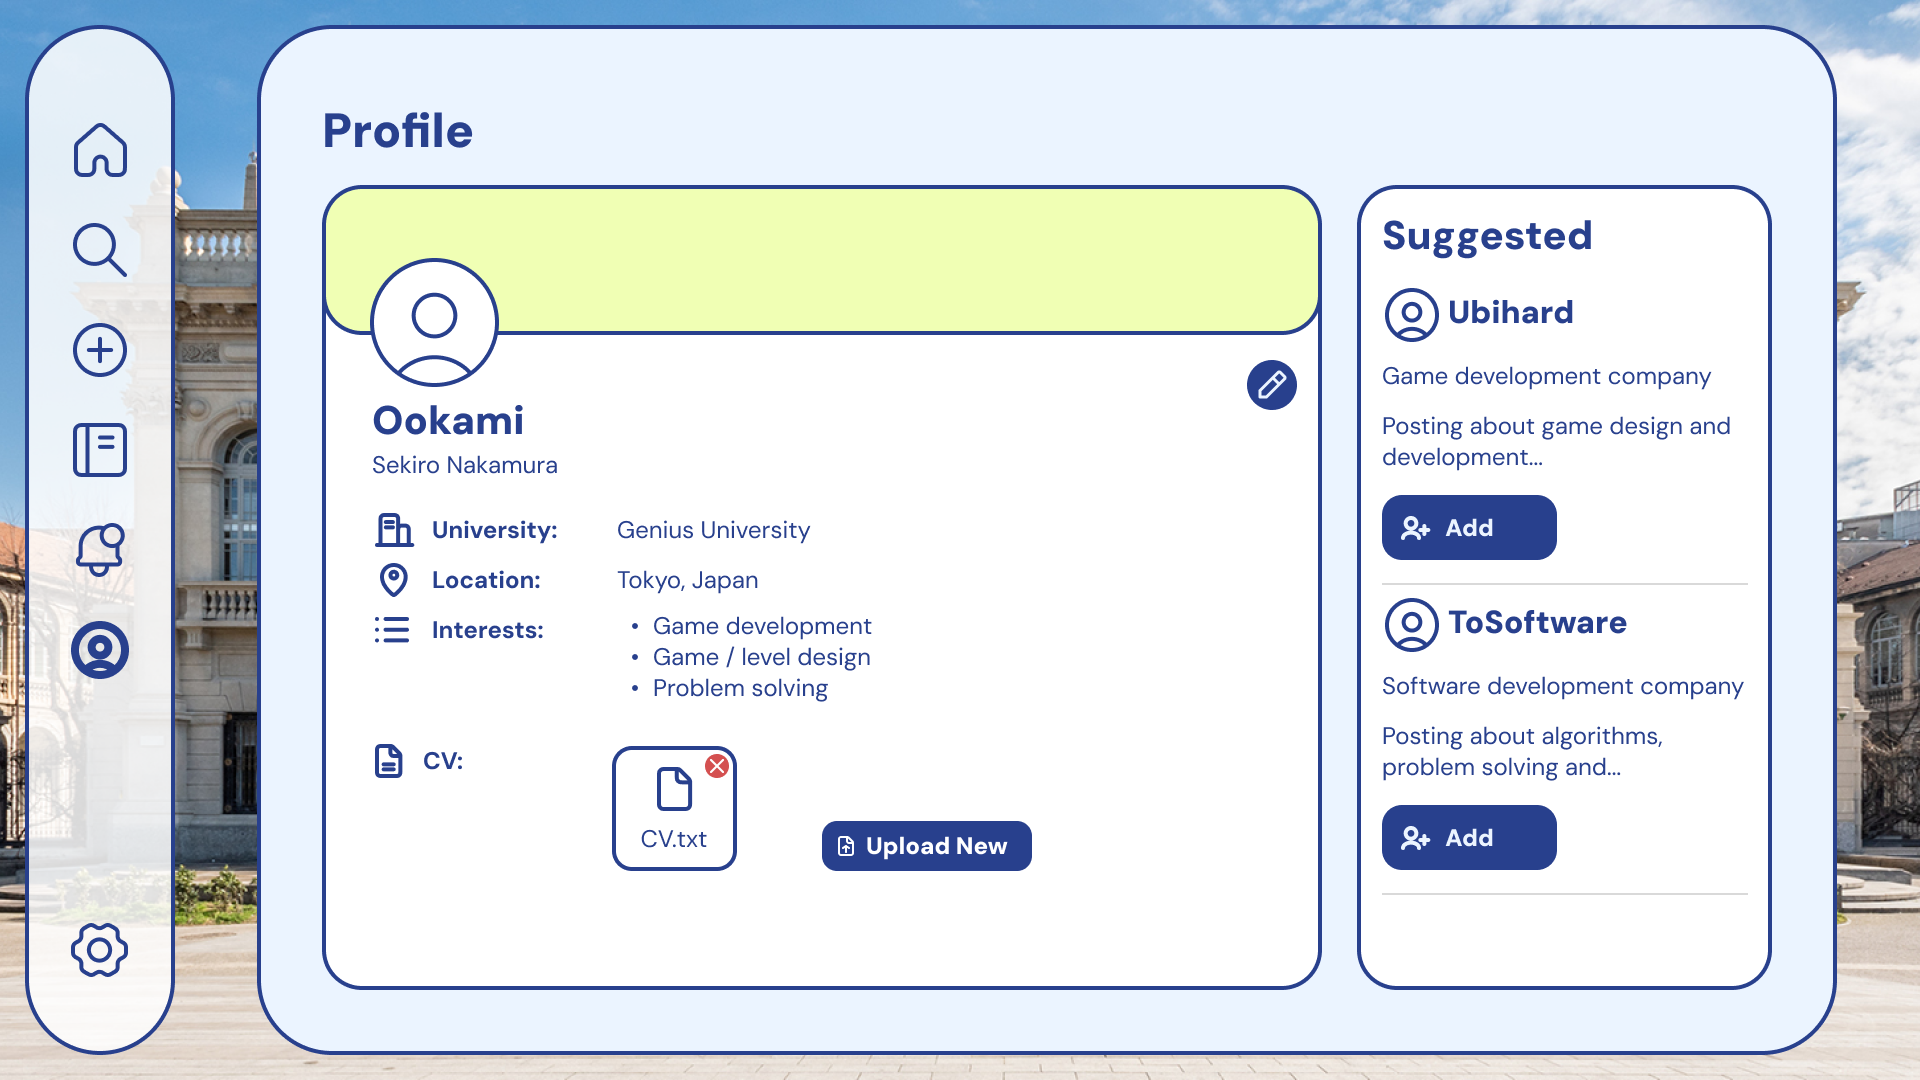
\includegraphics[width=\textwidth]{Images/Profile}
\caption{Student profile prototype page}\label{Student Profile}
\end{figure}
The picture [\ref{Student Profile}] shows the prototype of the profile page of a user logged in as a student. On the left, there is the section containing all the information provided by the user, and through the pencil button on the right, the user can modify the information. On the bottom there is the CV section. By clicking the file icon it opens the file allowing the user to check if the uploaded file is correct, otherwise the button on the right allows to upload a different file.\\
On the right side of the picture there is the "Suggested" area that show all the companies that might interest the user based on his interests.
\newpage
\large{\textbf{Notifications page}}
\begin{figure}[H]
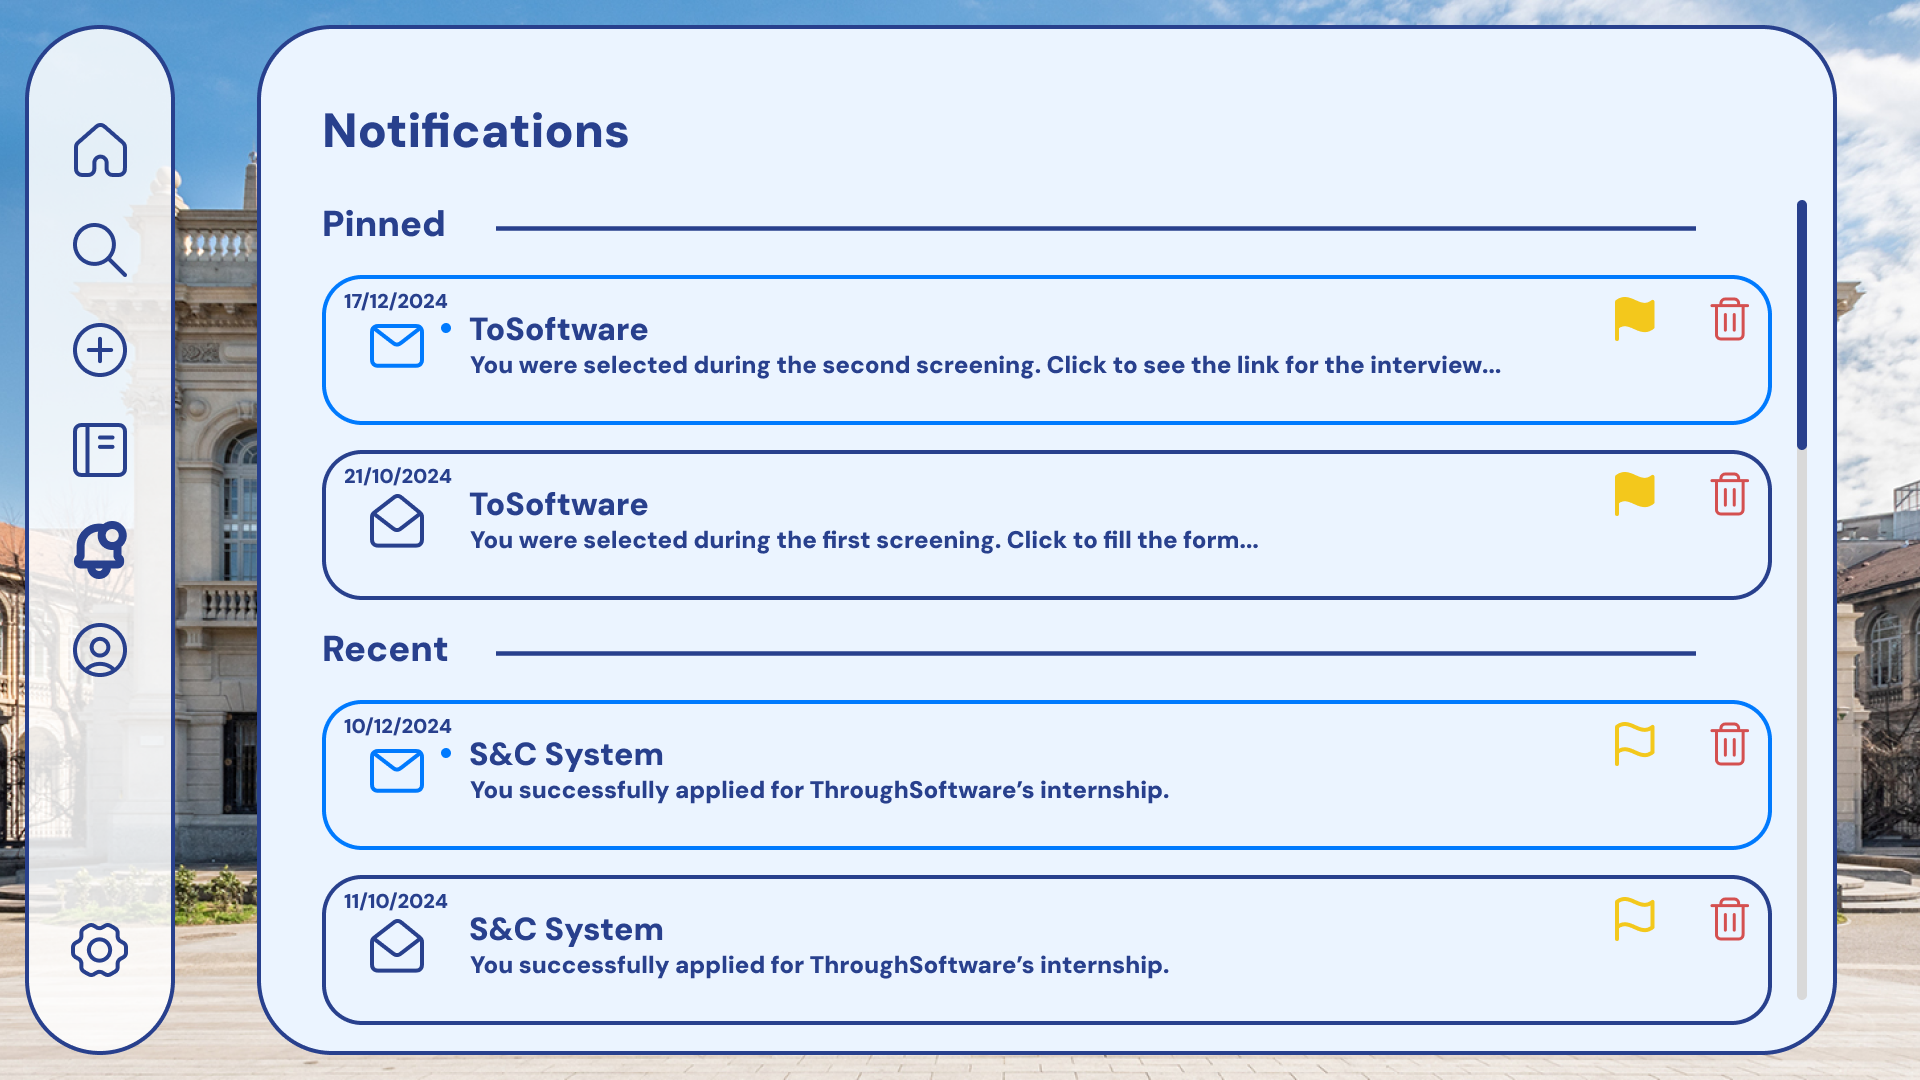
\includegraphics[width=\textwidth]{Images/Notifications}
\caption{Notifications prototype page}\label{Notifications}
\end{figure}
The picture [\ref{Notifications}] shows the prototype of the notifications page and is show to all three user categories. In general all notifications shown in the page render only a part of the whole message, and clicking on it allows the user to open a page that shows the whole text. In addition, notifications can be pinned to be always shown on top in their specific section by clicking on the yellow flag, or can be also permanently deleted by clicking on the trash can.
\newpage
\large{\textbf{Search page}}
\begin{figure}[H]
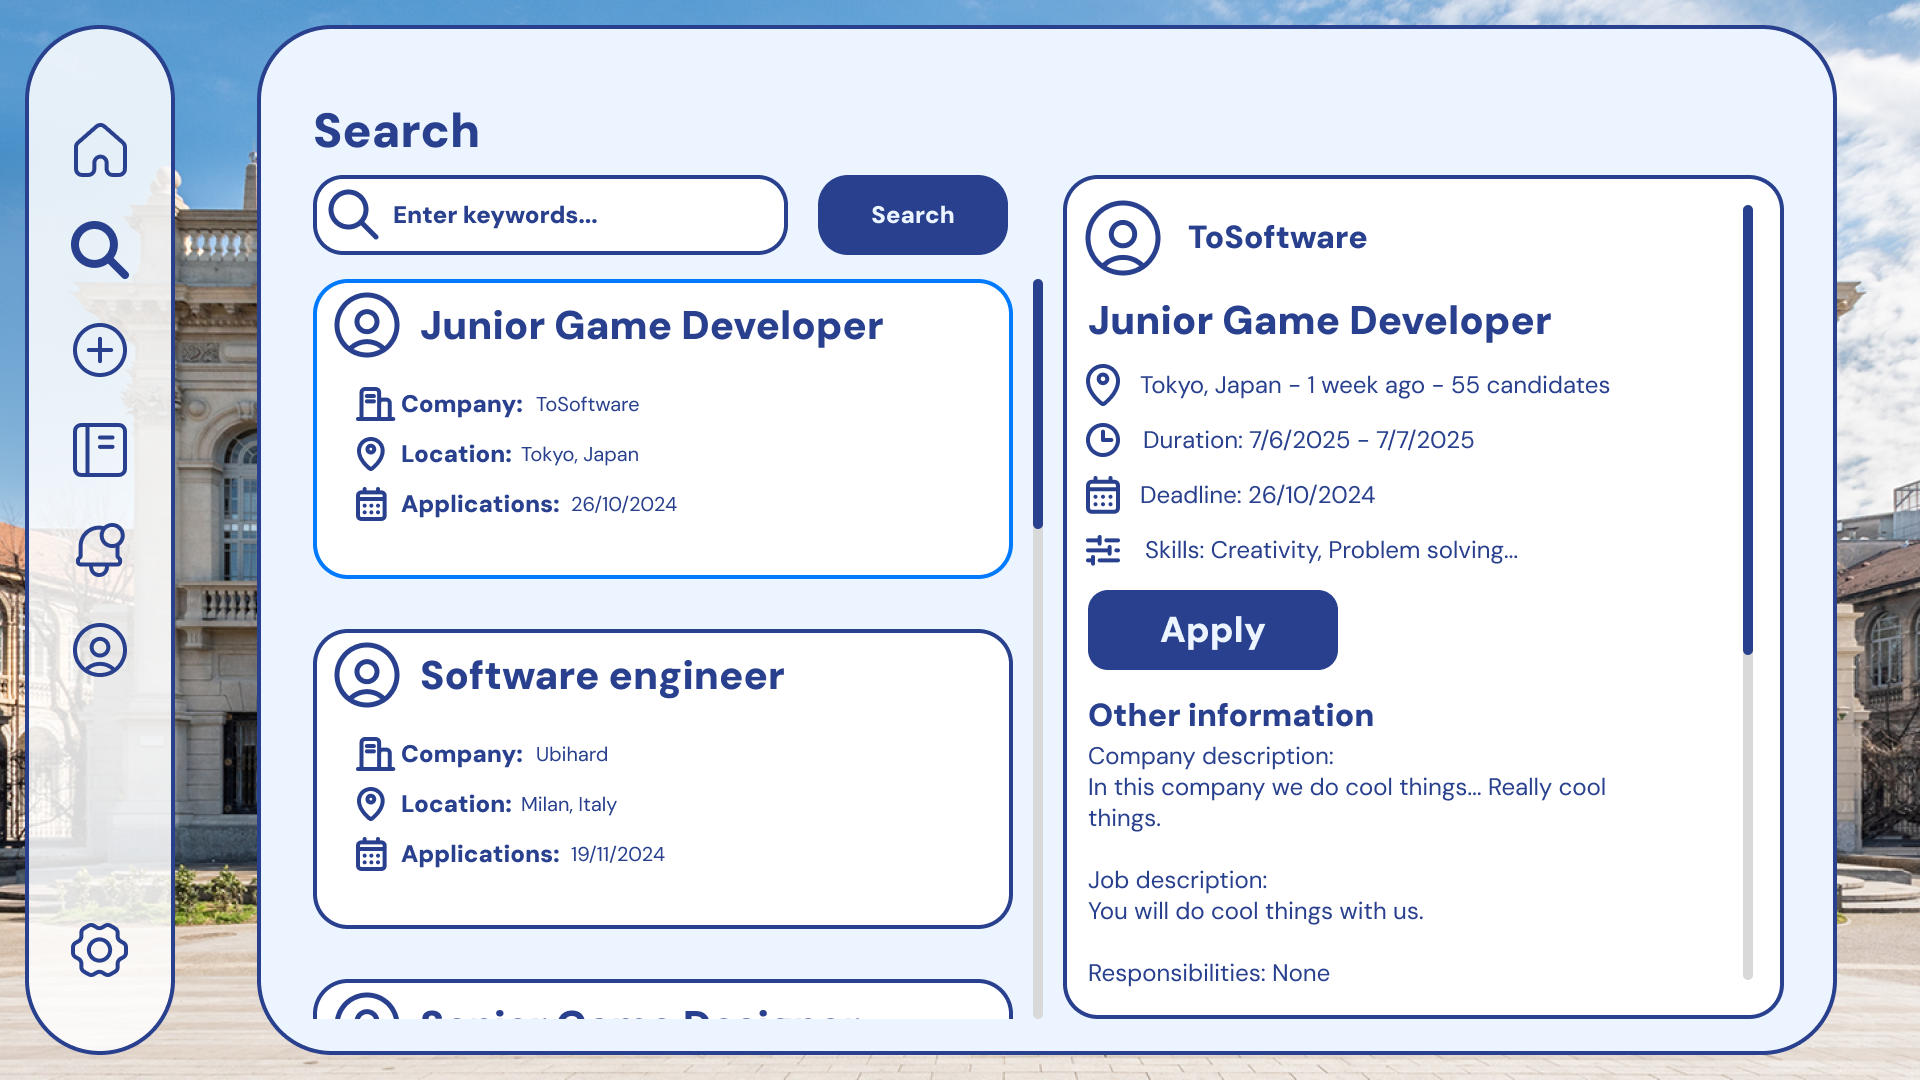
\includegraphics[width=\textwidth]{Images/Search}
\caption{Search prototype page}\label{Search}
\end{figure}
The picture [\ref{Search}] shows the prototype of the search page, that allow students to proactively search for internship by entering keywords in the search bar.\\
Right after searching the keywords the internship found are displayed on the left side and only show the basic details. By clicking on the desired internship, all the additional information entered by the company are displayed on the right side. Only when visualizing the details of an internship it is possible to apply for said offer through a dedicated button.
\newpage
\large{\textbf{Form creation page}}
\begin{figure}[H]
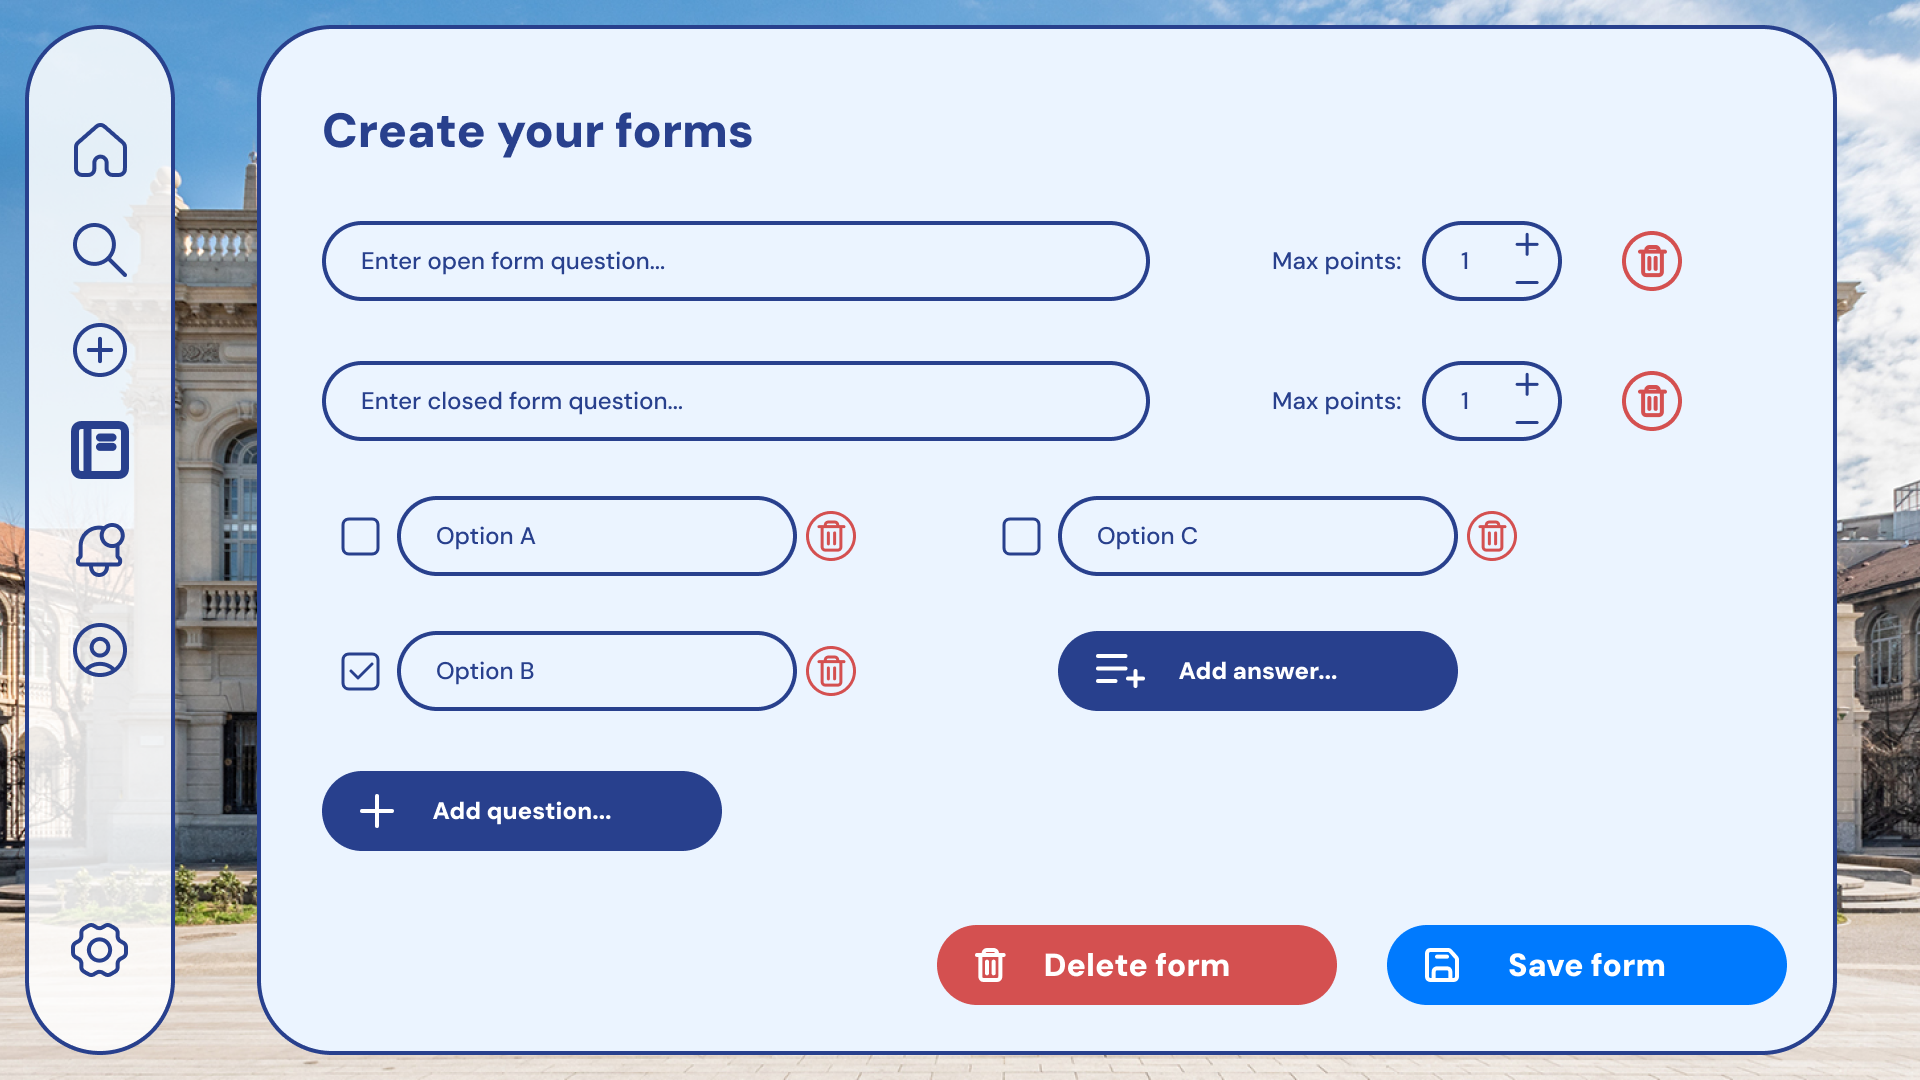
\includegraphics[width=\textwidth]{Images/Create form}
\caption{Form creation prototype page}\label{Form}
\end{figure}
The picture [\ref{Form}] shows the prototype of the form creation page that allows only companies to create custom forms for the candidates to fill during an application. In the form can be added two different types of questions: open and closed.\\
Open question only require the question text and the number of maximum point. \\
The closed ones not only require the question text and the maximum points like the open ones, but they also need the options the candidates have to choose from. Each option can be either deleted, marked as correct with the checkbox on the left, or can have its text changed. In addition the company can choose to add more options to the closed question with the \textit{"Add answer..."} button. \\
Lastly the company can decide to either add questions with the \textit{"Add question..."} button or delete them with the trash can icon on the right.\\
Once the form has been completed it can be saved or deleted by using the dedicated buttons.

\newpage

\large{\textbf{Home page}}
\begin{figure}[H]
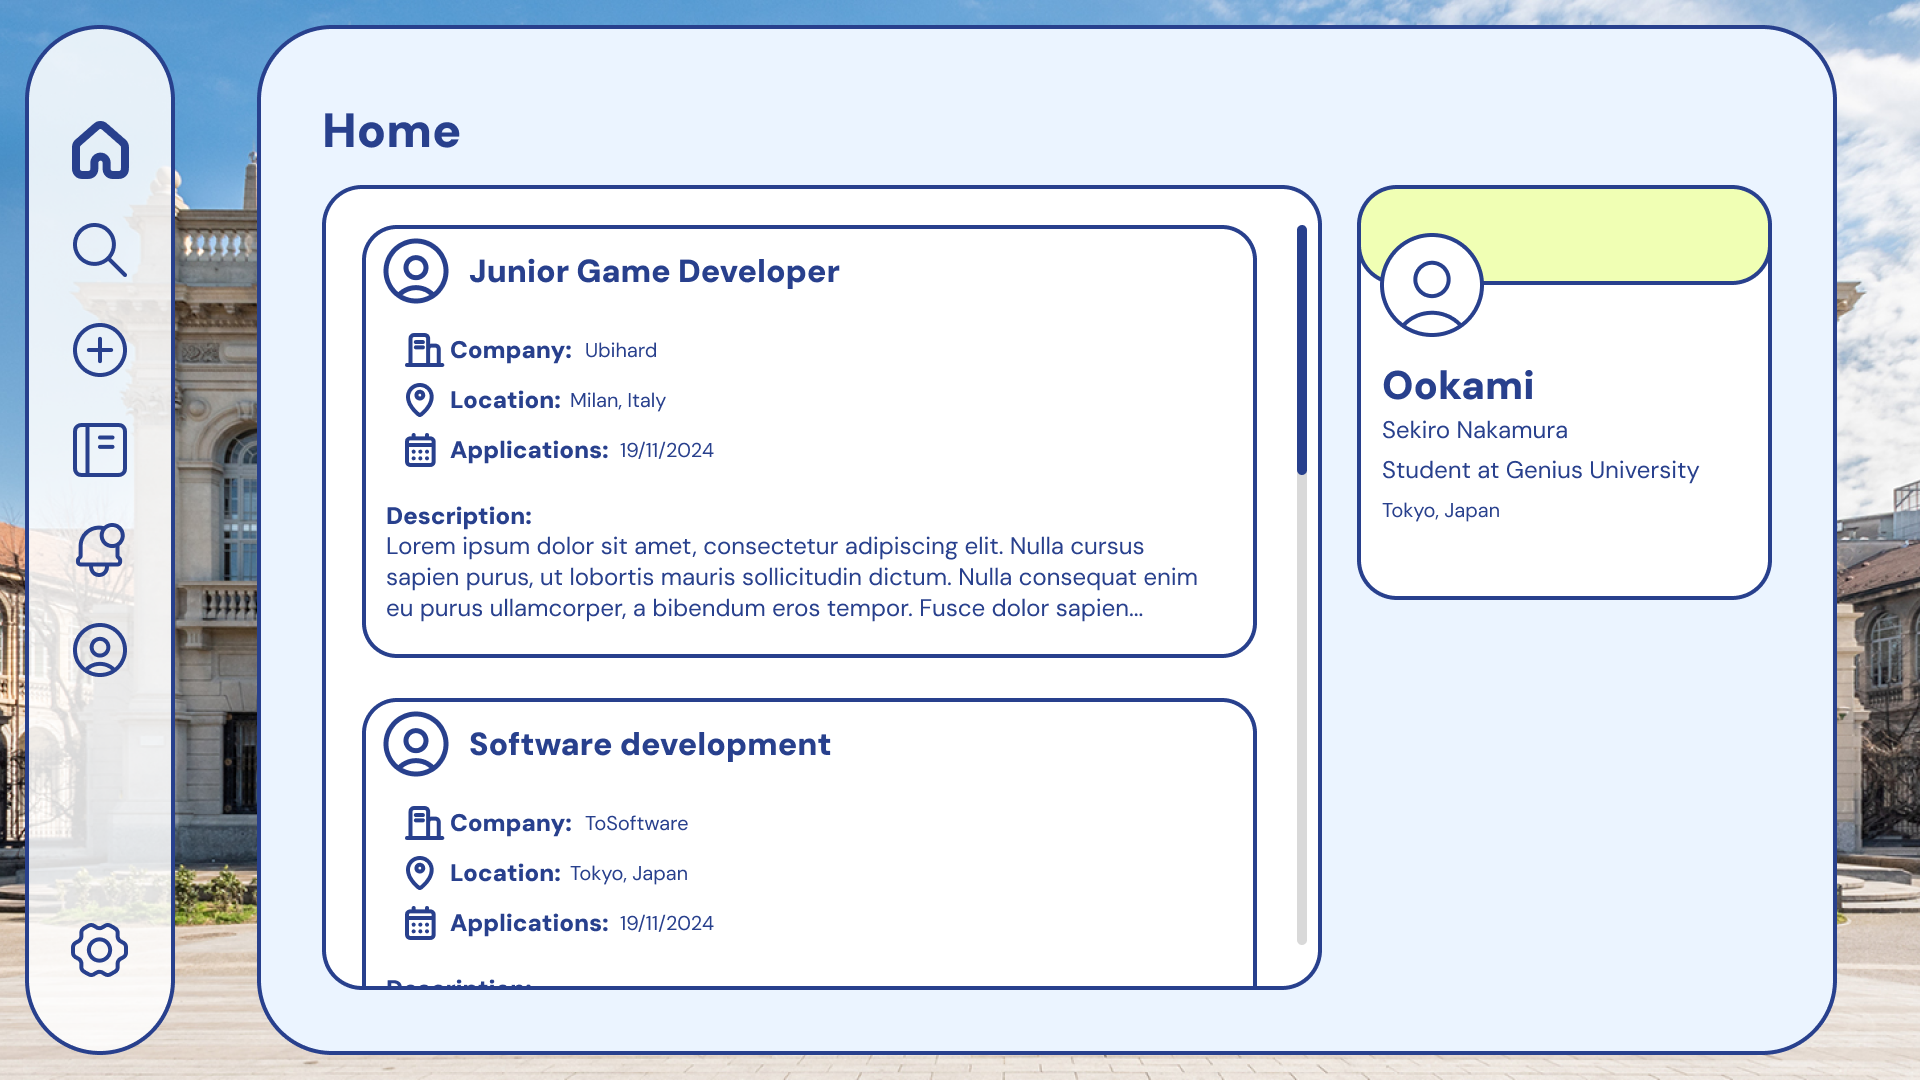
\includegraphics[width=\textwidth]{Images/Home}
\caption{Home prototype page}\label{Home}
\end{figure}
The picture [\ref{Home}] shows the prototype of the home page that allows students to see all the available internships posted by various companies.\\
The section on the left shows all the internships and by interacting with them the student can access a page that shows more details about the post and apply for the internship.\\
On the right there is a panel that shows the basic data regarding the user that is currently logged in.

\newpage

\large{\textbf{Internship creation page}}
\begin{figure}[H]
\includegraphics[width=\textwidth]{Images/Create internship}
\caption{Internship creation prototype page}\label{Create internship}
\end{figure}
The picture [\ref{Create internship}] shows the prototype of the page that allows companies to create and post about an internship.\\
In this page the company can add all the required information that allows the system to select the suitable students and notify them.

\newpage

\section{Requirement traceability}
In this section we are gonna look back at the goals and requirements described in the RASD and map them to the components created in the second chapter of this document. To make it easier to read we wrote again the goals followed by their already mapped requirements and then we added the components.\\
As we will see each goal is mapped to a single specific component of a subsystem since they were created with this exact purpose to ensure that each component would have a set of task to perform within a single context, providing as much modularity as possible.

\begin{table}[H]
\begin{tabular}{| p{0.3\textwidth} | p{0.64\textwidth} |}
\hline
\rowcolor{Gray1}
\textbf{G1} & \textbf{Student can create account} \\
\hline
\rowcolor{Gray2}
RA1 & The platform shall allow users to register \\
\hline
 & Components mapped to the requirements:
\begin{itemize}
\item Account Management
 	\begin{itemize}
 	\item Student Manager
 	\end{itemize}
\end{itemize} \\
\hline
\end{tabular}
\end{table}

\begin{table}[H]
\begin{tabular}{| p{0.3\textwidth} | p{0.64\textwidth} |}
\hline
\rowcolor{Gray1}
\textbf{G2} & \textbf{Company can create an account} \\
\hline
\rowcolor{Gray2}
RA1 & The platform shall allow users to register \\
\hline
 & Components mapped to the requirements:
\begin{itemize}
\item Account Management
 	\begin{itemize}
 	\item Company Manager
 	\end{itemize}
\end{itemize} \\
\hline
\end{tabular}
\end{table}

\begin{table}[H]
\begin{tabular}{| p{0.3\textwidth} | p{0.64\textwidth} |}
\hline
\rowcolor{Gray1}
\textbf{G2} & \textbf{Users can update their accounts} \\
\hline
\rowcolor{Gray2}
RA3 & The platform shall allow users to update their existing account \\
\hline
 & Components mapped to the requirements:
\begin{itemize}
\item Account Management
 	\begin{itemize}
 	\item Student Manager
	\item Company Manager
 	\end{itemize}
\end{itemize} \\
\hline
\end{tabular}
\end{table}

\begin{table}[H]
\begin{tabular}{| p{0.3\textwidth} | p{0.64\textwidth} |}
\hline
\rowcolor{Gray1}
\textbf{G4} & \textbf{Companies can create internships} \\
\hline
\rowcolor{Gray2}
RI1 & The platform must allow companies to create internships \\
\hline
 & Components mapped to the requirements:
\begin{itemize}
\item Internship Management
 	\begin{itemize}
 	\item Manage Internship
 	\end{itemize}
\end{itemize} \\
\hline
\end{tabular}
\end{table}

\newpage

\begin{table}[H]
\begin{tabular}{| p{0.3\textwidth} | p{0.64\textwidth} |}
\hline
\rowcolor{Gray1}
\textbf{G5} & \textbf{Students can view all available internships} \\
\hline
\rowcolor{Gray2}
RI2 & The platform must allow students to view all available internships \\
\hline
\rowcolor{Gray2}
RI3 & The platform must allow students to search between the available internship \\
\hline
 & Components mapped to the requirements:
\begin{itemize}
\item Internship Management
 	\begin{itemize}
 	\item Manage Internship
 	\end{itemize}
\end{itemize} \\
\hline
\end{tabular}
\end{table}

\begin{table}[H]
\begin{tabular}{| p{0.3\textwidth} | p{0.64\textwidth} |}
\hline
\rowcolor{Gray1}
\textbf{G6} & \textbf{Companies can create forms for students to fill} \\
\hline
\rowcolor{Gray2}
RF1 & The platform shall allow companies to create custom forms \\
\hline
\rowcolor{Gray2}
RF2 & The platform shall allow companies to save created forms for later use in an internship selection process \\
\hline
 & Components mapped to the requirements:
\begin{itemize}
\item Internship Management
 	\begin{itemize}
 	\item Form Management
 	\end{itemize}
\end{itemize} \\
\hline
\end{tabular}
\end{table}

\begin{table}[H]
\begin{tabular}{| p{0.3\textwidth} | p{0.64\textwidth} |}
\hline
\rowcolor{Gray1}
\textbf{G7} & \textbf{Recommendation system} \\
\hline
\rowcolor{Gray2}
RN1 & The platform shall notify students when an internship suitable for them has been posted \\
\hline
 & Components mapped to the requirements:
\begin{itemize}
\item Internship Management
 	\begin{itemize}
 	\item Manage Internship $\rightarrow$ \textit{findCompatibleStudents()}
 	\end{itemize}
\end{itemize} \\
\hline
\end{tabular}
\end{table}

\begin{table}[H]
\begin{tabular}{| p{0.3\textwidth} | p{0.64\textwidth} |}
\hline
\rowcolor{Gray1}
\textbf{G8} & \textbf{Students can apply for the internships} \\
\hline
\rowcolor{Gray2}
RI4 & The platform must allow students to apply for any available internship \\
\hline
 & Components mapped to the requirements:
\begin{itemize}
\item Internship Management
 	\begin{itemize}
 	\item Manage Internship
 	\end{itemize}
\end{itemize} \\
\hline
\end{tabular}
\end{table}

\newpage

\begin{table}[H]
\begin{tabular}{| p{0.3\textwidth} | p{0.64\textwidth} |}
\hline
\rowcolor{Gray1}
\textbf{G9} & \textbf{Form evaluation} \\
\hline
\rowcolor{Gray2}
RN7 & The platform shall send companies the list of candidates at the end of the application deadline \\
\hline
\rowcolor{Gray2}
RF3 & The platform shall allow companies to send the candidates that passed the first screening the form for the second screening \\
\hline
\rowcolor{Gray2}
RF4 & The platform shall allow students to fill and submit the application form \\
\hline
\rowcolor{Gray2}
RF5 & The platform shall allow companies to evaluate a submitted form by grading each question \\
\hline
 & Components mapped to the requirements:
\begin{itemize}
\item Internship Management
 	\begin{itemize}
 	\item Form Management
 	\end{itemize}
\end{itemize} \\
\hline
\end{tabular}
\end{table}

\begin{table}[H]
\begin{tabular}{| p{0.3\textwidth} | p{0.64\textwidth} |}
\hline
\rowcolor{Gray1}
\textbf{G10} & \textbf{Ranking candidates} \\
\hline
\rowcolor{Gray2}
RN2 & The platform shall notify students of the result of the first screening \\
\hline
\rowcolor{Gray2}
RN3 & The platform shall notify students of the result of the second screening \\
\hline
\rowcolor{Gray2}
RN4 & The platform shall notify students of the final result of the application \\
\hline
 & Components mapped to the requirements:
\begin{itemize}
\item Internship Management
 	\begin{itemize}
 	\item Internship selection $\rightarrow$ \textit{getRanking()}
 	\end{itemize}
\end{itemize} \\
\hline
\end{tabular}
\end{table}

\begin{table}[H]
\begin{tabular}{| p{0.3\textwidth} | p{0.64\textwidth} |}
\hline
\rowcolor{Gray1}
\textbf{G11} & \textbf{Users can provide feedbacks} \\
\hline
\rowcolor{Gray2}
RN5 & The platform shall notify students/companies to fill a feedback form after the end of the internship \\
\hline
\rowcolor{Gray2}
RR1 & The platform shall allow students and companies to write a feedback at the end of an internship \\
\hline
 & Components mapped to the requirements:
\begin{itemize}
\item Internship Management
 	\begin{itemize}
 	\item Feedback
 	\end{itemize}
\end{itemize} \\
\hline
\end{tabular}
\end{table}

\newpage

\begin{table}[H]
\begin{tabular}{| p{0.3\textwidth} | p{0.64\textwidth} |}
\hline
\rowcolor{Gray1}
\textbf{G12} & \textbf{Complaints management} \\
\hline
\rowcolor{Gray2}
RI5 & The platform shall allow students/companies involved in an internship to complain about the other party \\
\hline
\rowcolor{Gray2}
RN6 & The platform shall notify universities whenever a complaint is filed involving one of their students \\
\hline
\rowcolor{Gray2}
RR2 & The platform shall allow students and companies involved in an internship to write complaints regarding the other party \\
\hline
\rowcolor{Gray2}
RR3 & The platform shall allow universities to read all complaints that involve their students \\
\hline
 & Components mapped to the requirements:
\begin{itemize}
\item Internship Management
 	\begin{itemize}
 	\item Complaints
 	\end{itemize}
\end{itemize} \\
\hline
\end{tabular}
\end{table}

\newpage

\section{Implementation, Integration, and Test Plan}
This chapter explains how to implement, integrate, and plan the tests for the application designed in this document. The chapter is divided into two fundamental parts. The first one (\textbf{Components Development}) describes how the components designed in this document should be implemented, integrated, and tested. The second one (\textbf{System Testing}) explains how testing for the system as a whole should be executed.

\subsection{Components Development}
The system is divided into the following subsystems:
\begin{itemize}
\item Web Browser
\item Mobile Device
\item Account Management
\item Internship Management
\end{itemize}

The first two are designed for the client side of the application, while the latter two handle the server-side functionalities, including data and application layer management, as detailed in Section 2. These subsystems must be implemented, tested, and integrated using a \textbf{bottom-up} approach. To ensure development progresses as intended, we provide a prioritized order for development based on dependencies. While client and server-side components can be developed in parallel, final integration and testing will be performed together. 

\textbf{Development Order and Difficulty:}

\begin{table}[H]
\centering
\begin{tabular}{|p{0.3\textwidth}|p{0.3\textwidth}|p{0.3\textwidth}|}
\hline
\textbf{Order} & \textbf{Stage} & \textbf{Difficulty} \\
\hline
1 & Account Management & Medium \\
\hline
2 & Internship Management & High \\
\hline
3 & Web Browser Interface & Low \\
\hline
4 & Mobile Device Interface & Medium \\
\hline
\end{tabular}
\caption{Development stages and difficulty levels for system components.}
\end{table}

\textbf{Implementation and Testing Plan:}
\begin{itemize}
    \item \textbf{Account Management:} Focuses on user authentication and the creation/update of accounts. Unit tests will validate functionality, followed by integration tests with the database, since it's mostly composed of only a few components that depend on each other (student/company manager and authentication system) it shouldn't pose any problems and the aforementioned components can be implemented in parallel with the use of suitable drivers for the simulation of the required interfaces. Testing scenarios will include edge cases for password complexity, role-based access permissions, and session management.
    \item \textbf{Internship Management:} Handles internship tracking, student assignments, and reporting. It is composed of many different interdependent components some of which are of critical importance (e.g.: Recommendation System, Notification System) and should therefor be given high priority, a parallel implementation plan can also be adopted in this case with the use of drivers/stubs whenever needed but should be proceeded with utmost care and attention since this subsystem represents the core funcionality of the software-to-be. For what regards the testing, the subsystem will undergo rigorous testing, including boundary tests for data handling and stress tests for performance. Additional checks will ensure data integrity during concurrent user operations.
    \item \textbf{Web Browser Interface:} Ensures compatibility across major browsers and responsive design. Functional tests will verify usability and ease of navigation. Some additional user tests will help identify areas for improvement with regards to the UI and UX.
    \item \textbf{Mobile Device Interface:} Ensures smooth operation on Android and iOS platforms. Device-specific tests and cross-platform validations will be conducted, covering offline functionalities and seamless synchronization with the server, any performance/functional requirements not met can be immediately discovered through tests.
\end{itemize}


\subsection{System Testing}
System testing involves validating the entire application as an integrated unit to ensure all components function together seamlessly. The following phases will be executed:

\begin{itemize}
    \item \textbf{Integration Testing:} Verifies the correct interaction between subsystems. Test cases will focus on data flow, API interactions, and synchronization between client and server sides. Special attention will be given to handling exceptions and invalid requests or states of the user.
    \item \textbf{Functional Testing:} Ensures the system meets all specified requirements. Scenarios will include user login, internship application workflows, and report generation. Regression tests will be conducted to confirm that new updates do not introduce unintended already faced issues and bugs.
    \item \textbf{Performance Testing:} Evaluates system response under various loads. Stress and load tests will try to find bottlenecks in the system so that they can be fixed and adjusted. Metrics such as response time, throughput, and server utilization will be monitored.
    \item \textbf{User Acceptance Testing (UAT):} Conducted with end users to validate the system's functionality, usability, and compliance with expectations. Feedback collected during UAT will be analyzed for final adjustments before deployment.
\end{itemize}

This systematic approach ensures that the application is robust, reliable, and ready for deployment.

	
\newpage

\section{Effort spent}

\begin{itemize}

\item \textbf{Abdallah Alkhetiar}
\begin{table}[H]
\begin{tabular}{| >{\centering\arraybackslash}m{0.2\textwidth} || >{\centering\arraybackslash}m{0.2\textwidth} |}
\hline
\textbf{Chapter} & \textbf{Effort} \\
\hline
1 & 0 h \\
\hline
2 & 0 h \\
\hline
3 & 0 h \\
\hline
4 & 0 h \\
\hline
5 & 0 h \\
\hline
\end{tabular}
\end{table}

\vspace{1\baselineskip}

\item \textbf{Daniel Bonardi}
\begin{table}[H]
\begin{tabular}{| >{\centering\arraybackslash}m{0.2\textwidth} || >{\centering\arraybackslash}m{0.2\textwidth} |}
\hline
\textbf{Chapter} & \textbf{Effort} \\
\hline
1 & 0 h \\
\hline
2 & 0 h \\
\hline
3 & 0 h \\
\hline
4 & 0 h \\
\hline
5 & 0 h \\
\hline
\end{tabular}
\end{table}

\end{itemize}

\newpage

\section{References}
\textbf{N-tier architectures}\\
\href{https://dev.to/3bdelrahman/understanding-layers-tiers-and-n-tier-architecture-in-application-development-1hlb}{\textcolor{blue}{https://dev.to/3bdelrahman}}\\
\href{https://blog.nginx.org/blog/time-to-move-to-a-four-tier-application-architecture#:~:text=Forrester\%27s\%20Four‑Tier\%20Engagement\%20Platform,\%2C\%20aggregation\%2C\%20and\%20services\%20layers.}{\textcolor{blue}{https://blog.nginx.org/blog}}\\
\href{https://www.klipfolio.com/resources/data-stack/integration-layer}{\textcolor{blue}{https://www.klipfolio.com}} \\
\textbf{Elasticsearch} \\
\href{https://www.elastic.co}{\textcolor{blue}{https://elastic.co}} \\
\textbf{OAuth2.0} \\
\href{https://auth0.com/intro-to-iam/what-is-oauth-2}{\textcolor{blue}{https://auth0.com}}

\end{document}
